\RequirePackage[l2tabu,orthodox]{nag}

% TODO: decide if one-sided/two-sided
%\documentclass[headsepline,footsepline,footinclude=false,fontsize=11pt,paper=a4,listof=totoc,bibliography=totoc,BCOR=12mm,DIV=12]{scrbook} % two-sided
\documentclass[headsepline,footsepline,footinclude=false,oneside,fontsize=11pt,paper=a4,listof=totoc,bibliography=totoc]{scrbook} % one-sided

% TODO: change citation style in settings
\PassOptionsToPackage{table,svgnames,dvipsnames}{xcolor}

\usepackage[utf8]{inputenc}
\usepackage[T1]{fontenc}
\usepackage[sc]{mathpazo}
\usepackage[ngerman,american]{babel}
\DeclareUnicodeCharacter{200B}{}
\usepackage[autostyle]{csquotes}
\usepackage[%
  backend=biber,
  url=false,
  style=alphabetic,
  maxnames=4,
  minnames=3,
  maxbibnames=99,
  giveninits,
  uniquename=init]{biblatex} % TODO: adapt citation style
\usepackage{graphicx}
\usepackage{scrhack} % necessary for listings package
\usepackage{listings}
\usepackage{lstautogobble}
\usepackage{tikz}
\usepackage{pgfplots}
\usepackage{pgfplotstable}
\usepackage{booktabs}
\usepackage[final]{microtype}
\usepackage{caption}
\usepackage{float}
\usepackage{enumitem}
\usepackage{longtable}
\usepackage{adjustbox} % preamble
\usepackage[hidelinks]{hyperref} % hidelinks removes colored boxes around references and links

\usetikzlibrary{positioning, arrows.meta}
\bibliography{bibliography}

\setkomafont{disposition}{\normalfont\bfseries} % use serif font for headings
\linespread{1.05} % adjust line spread for mathpazo font

% Add table of contents to PDF bookmarks
\BeforeTOCHead[toc]{{\cleardoublepage\pdfbookmark[0]{\contentsname}{toc}}}

% Define TUM corporate design colors
% Taken from http://portal.mytum.de/corporatedesign/index_print/vorlagen/index_farben
\definecolor{TUMBlue}{HTML}{0065BD}
\definecolor{TUMSecondaryBlue}{HTML}{005293}
\definecolor{TUMSecondaryBlue2}{HTML}{003359}
\definecolor{TUMBlack}{HTML}{000000}
\definecolor{TUMWhite}{HTML}{FFFFFF}
\definecolor{TUMDarkGray}{HTML}{333333}
\definecolor{TUMGray}{HTML}{808080}
\definecolor{TUMLightGray}{HTML}{CCCCC6}
\definecolor{TUMAccentGray}{HTML}{DAD7CB}
\definecolor{TUMAccentOrange}{HTML}{E37222}
\definecolor{TUMAccentGreen}{HTML}{A2AD00}
\definecolor{TUMAccentLightBlue}{HTML}{98C6EA}
\definecolor{TUMAccentBlue}{HTML}{64A0C8}

% Settings for pgfplots
\pgfplotsset{compat=newest}
\pgfplotsset{
  % For available color names, see http://www.latextemplates.com/svgnames-colors
  cycle list={TUMBlue\\TUMAccentOrange\\TUMAccentGreen\\TUMSecondaryBlue2\\TUMDarkGray\\},
}

% Settings for lstlistings
\lstset{%
  basicstyle=\ttfamily,
  columns=fullflexible,
  autogobble,
  keywordstyle=\bfseries\color{TUMBlue},
  stringstyle=\color{TUMAccentGreen}
}

\setlength{\parskip}{1em}  % space between paragraphs
\setlength{\parindent}{0pt}  % no indentation


% TODO: change thesis information
\newcommand*{\getUniversity}{Technische Universität München}
\newcommand*{\getFaculty}{Department of Informatics}
\newcommand*{\getTitle}{AI-Assisted Domain Modeling: Enhanced Bounded Context Extraction with LLMs}
\newcommand*{\getTitleGer}{KI-unterstützte Domänenmodellierung: Verbesserte Extraktion von Bounded Contexts mit LLMs}
\newcommand*{\getAuthor}{Husein Jusic}
\newcommand*{\getDoctype}{Bachelor's Thesis in Informatics}
\newcommand*{\getSupervisor}{Tobias Eisenreich}
\newcommand*{\getAdvisor}{Michael Krinninger}
\newcommand*{\getSubmissionDate}{\today}
\newcommand*{\getSubmissionLocation}{Munich}

\begin{document}

% Set page numbering to avoid "destination with the same identifier has been already used" warning for cover page.
% (see https://en.wikibooks.org/wiki/LaTeX/Hyperlinks#Problems_with_Links_and_Pages).
\pagenumbering{alph}
\begin{titlepage}
  % HACK for two-sided documents: ignore binding correction for cover page.
  % Adapted from Markus Kohm's KOMA-Script titlepage=firstiscover handling.
  % See http://mirrors.ctan.org/macros/latex/contrib/koma-script/scrkernel-title.dtx,
  % \maketitle macro.
  \oddsidemargin=\evensidemargin\relax
  \textwidth=\dimexpr\paperwidth-2\evensidemargin-2in\relax
  \hsize=\textwidth\relax

  \centering

  \IfFileExists{logos/tum.png}{%
    
\includegraphics[height=20mm]{logos/tum.png}
  }{%
    \vspace*{20mm}
  }

  \vspace{5mm}
  {\huge\MakeUppercase{\getFaculty{}}}\\

  \vspace{5mm}
  {\large\MakeUppercase{\getUniversity{}}}\\

  \vspace{20mm}
  {\Large \getDoctype{}}

  \vspace{15mm}
  {\huge\bfseries \getTitle{}}

  \vspace{15mm}
  {\LARGE \getAuthor{}}

  \IfFileExists{logos/faculty.pdf}{%
    \vfill{}
    \includegraphics[height=20mm]{logos/faculty.pdf}
  }{}
\end{titlepage}


\frontmatter{}

\begin{titlepage}
  \centering

  \IfFileExists{logos/tum.pdf}{%
    
\includegraphics[height=20mm]{logos/tum.pdf}
  }{%
    \vspace*{20mm}
  }

  \vspace{5mm}
  {\huge\MakeUppercase{\getFaculty{}}}\\

  \vspace{5mm}
  {\large\MakeUppercase{\getUniversity{}}}\\

  \vspace{20mm}
  {\Large \getDoctype{}}

  \vspace{15mm}
  {\huge\bfseries \getTitle{} \par}

  \vspace{10mm}
  {\huge\bfseries \foreignlanguage{ngerman}{\getTitleGer{}} \par}

  \vspace{15mm}
  \begin{tabular}{l l}
    Author:          & \getAuthor{} \\
    Supervisor:      & \getSupervisor{} \\
    Advisor:         & \getAdvisor{} \\
    Submission Date: & \getSubmissionDate{} \\
  \end{tabular}

  \IfFileExists{logos/faculty.pdf}{%
    \vfill{}
    \includegraphics[height=20mm]{logos/faculty.pdf}
  }{}
\end{titlepage}

\thispagestyle{empty}
\vspace*{0.8\textheight}
\noindent
I confirm that this \MakeLowercase{\getDoctype{}} is my own work and I have documented all sources and material used.

\vspace{15mm}
\noindent
\getSubmissionLocation{}, \getSubmissionDate{} \hspace{50mm} \getAuthor{}

\cleardoublepage{}

\addcontentsline{toc}{chapter}{Acknowledgments}
\thispagestyle{empty}

\vspace*{20mm}

\begin{center}
{\usekomafont{section} Acknowledgments}
\end{center}

\vspace{10mm}

%TODO: Acknowledgments

\cleardoublepage{}

\chapter{\abstractname}


This thesis explores the application of Large Language Models (LLMs) to enhance domain modeling in software architecture, specifically focusing on the extraction of bounded contexts as defined by Domain-Driven Design (DDD). Traditional domain modeling is a time-consuming and expertise-driven process, often leading to suboptimal architectures under tight deadlines. This research investigates how AI can assist in decomposing complex monolithic systems into modular, maintainable components.

A case study was conducted with FTAPI Software GmbH, a company facing the challenge of modernizing its legacy monolithic architecture. A five-phase, prompt-driven workflow was developed to guide LLMs through a structured analysis, including ubiquitous language extraction, event storming, bounded context identification, aggregate design, and technical architecture mapping. This methodology was applied to two distinct domains: SecuRooms, a well-defined and previously modularized system serving as a benchmark, and SecuMails, a complex monolithic system targeted for modernization.

The results show that LLMs can effectively generate viable bounded contexts and domain models that closely align with those created by experienced human architects, especially for domains with clear requirements like SecuRooms. For the more entangled SecuMails monolith, the LLM proposals provided a valuable starting point but struggled to capture implicit business rules and historical technical debt. Expert interviews confirmed the value of the LLM as an "architectural sparring partner" that accelerates initial design, enforces systematic analysis, and offers unbiased perspectives.

The thesis concludes that a semi-automated approach, combining the analytical speed of LLMs with the contextual judgment of human experts, offers a highly effective strategy for software architecture design. This collaborative model enables a more thorough exploration of architectural candidates, ultimately leading to more robust and maintainable systems.
\microtypesetup{protrusion=false}
\tableofcontents{}
\microtypesetup{protrusion=true}

\mainmatter{}


\chapter{Introduction and Overview}\label{chapter:introduction}

\section{Motivation}
Software architecture design is a critical and challenging phase in the software development life cycle, particularly within larger Companies where systems are complex and must support extensive scalability requirements. As highlighted by Eisenreich et al. \autocite{eisenreich2024} designing domain models and software architectures is not only time-consuming but also significantly impacts the quality of service delivered by the resulting system. 

In practice, the architecture design process in enterprise environments is constrained by tight deadlines, limited resources and business pressure which often leads software architects to pick suboptimal solutions: either taking the first viable architecture design without deep exploration of alternatives or creating very simple architectures that satisfy the immediate requirements but without considering long-term quality attributes. This stands in contrast to the idealized approach where multiple architecture candidates would be created, thoroughly evaluated and compared before settling for the most suitable solution. 

The consequences of hastily constructed software architectures are well-documented in software engineering literature. Suboptimal architectures for example can lead to increased maintenance cost as analyzed by MacCormack et al. \autocite{MACCORMACK2016170}. Specifically for SaaS Companies these consequences can translate to competitive disadvantages as their business model depends on maintaining a robust software foundation. 

The recent quality advancements of LLMs present promising opportunities to address these challenges. Eisenreich et al. \cite{eisenreich2024} have proposed a vision for semi-automatically generating software architectures using artificial intelligence techniques, particularly LLMs, based on software requirements. Their approach suggests leveraging AI to generate domain models and multiple architecture candidates, followed by a manual evaluation and trade-off analysis of the created architectures. 

While their vision provides a valuable conceptual framework, its application specifically in large-scale software environments with lots of requirements remains unexplored. 

\section{Outlook}
This thesis aims to extend Eisenreich's vision by investigating how different LLMs can be utilized specifically in the context of large SaaS Software. We will conduct an empirical study with a SaaS Company - FTAPI Software GmbH. By focusing specifically on the domains of larger Software and conducting research within an actual enterprise environment, this thesis aims to provide insights into the applicability of AI-Assisted architecture design and the specific considerations required when applying these techniques in larger-scale software development contexts.

\section{Research Question and Objectives}

This thesis aims to explore and analyze how LLMs can be utilized in the industry with large requirement sets to help developers with creating and refining software architectures with large requirements sets

\begin{itemize}
    \item How effectively can Large Language Models (LLMs) identify and define viable bounded contexts that align with complex domain-specific requirements?
    \item To what extent do bounded contexts and domain models identified by LLMs compare in quality and applicability with those created by experienced DDD practitioners when analyzing complex application requirements?
\end{itemize}

\section{Structure}

This thesis is organized into eight chapters structured as follows:

\begin{description}
\item[Chapter~\ref{chapter:introduction}] introduces the research problem, presents the motivation for this work, and outlines the main contributions.

\item[Chapter~\ref{chapter:theoreticalbg}] provides the theoretical foundations necessary to understand the proposed approach.

\item[Chapter~\ref{chapter:relatedwork}] discusses related research and examines existing solutions to similar problems.

\item[Chapter~\ref{chapter:ftapi}] introduces the collaborating company and defines the specific business problem addressed in this thesis.

\item[Chapter~\ref{chapter:method}] describes the research methodology and approach taken to solve the identified problem.

\item[Chapter~\ref{chapter:implementation}] details the technical realization and implementation of the proposed solution.

\item[Chapter~\ref{chapter:results}] presents the experimental results and findings in an objective manner.

\item[Chapter~\ref{chapter:discussion}] critically analyzes these results, discusses their implications, and addresses the limitations of the proposed approach.
\end{description}
\chapter{Theoretical Background}\label{chapter:theoreticalbg}
In this chapter, we introduce the theoretical concepts fundamental to this thesis. We begin with Domain-Driven Design, which provides the architectural framework for our investigation into LLM-assisted bounded context extraction.

\section{Domain Driven Design}\label{sec:ddd}
Domain Driven Design (DDD) describes a process for software development that was introduced by Eric Evans in his seminal work "Domain-Driven Design: Tackling Complexity in the Heart of Software" \autocite{evans2004domain}. This methodology emphasizes creating software systems that accurately reflect and align with the business domain they serve. DDD is particularly valuable for complex systems with extensive requirements where business logic is continually evolving and changing.

The core philosophy of DDD centers on prioritizing the domain model over technical concerns, enabling software development teams to solve business problems instead of getting entangled in implementation details. This approach typically results in software that is more maintainable and closely aligned with business objectives. Empirical research supports this claim; for example, Özkan et al. \autocite{ddd-maintainability} conducted a case study demonstrating that DDD implementation significantly improved the maintainability metrics of a large-scale commercial software system compared to its previous architecture.

\subsection{Domain}
Evans provides a foundational definition of the term "domain" in his seminal work:
\begin{quote}
"Every software program relates to some activity or interest of its user. That subject area to which the user applies the program is the domain of the software."
\autocite[p.~4]{evans2004domain}
\end{quote}
Furthermore, he makes it clear that the domain represents more than just a subject area; it encompasses the entire business context within which a software system operates. It includes all the business rules, processes, workflows, terminology, and conceptual models that domain experts use when discussing and working within their field of expertise. Vernon \autocite[p.~17]{vernon2013implementing} further clarifies this by explaining that a domain is "a sphere of knowledge and activity around which the application logic revolves."

\subsection{Ubiquitous Language}
One of the core concepts of DDD is the development of a Ubiquitous Language. A Ubiquitous Language is a shared vocabulary that is consistently used by domain experts and the developers. This shared vocabulary improves communication, mitigates translation errors and improves communication between technical and non-technical stakeholders when discussing the business domain.

Vernon \autocite[p.~22]{vernon2013implementing} provides an example on how Ubiquitous Language directly affects code design. He presents three approaches to modeling a flu vaccination scenario, each reflecting a different level of domain understanding.

His example shown in Table~\ref{tab:ubiquitous-language-examples} demonstrates how the evolution of language directly impacts code structure and domain modeling. The progression from generic, technical language to precise, domain-aligned terminology, illustrates a fundamental principle: the language we use shapes the software we build.

Ubiquitous Language plays a crucial role in identifying and maintaining bounded contexts. Evans \autocite[p.~13]{Evans2003} emphasizes that "the model is the backbone of a language used by all team members", and this language serves as the primary indicator of context boundaries. When the same term carries different meanings or when communication requires translation between team members, these linguistic fractures often reveal the natural boundaries between bounded contexts.

Within a well-defined bounded context, every term has a single, precise meaning that all team members, both technical and domain experts, understand identically. This linguistic consistency prevents the subtle corruption of domain concepts that often occurs when boundaries are unclear. For instance, the term "customer" might mean a person with an active subscription in a billing context, while in a marketing context it could include prospects and past customers. These semantic differences signal the need for separate bounded contexts.

\begin{table}[htbp]
    \centering
    \begin{adjustbox}{max width=\textwidth}
    \begin{tabular}{|m{5cm}|m{9cm}|}
    \hline
    \rowcolor{gray!20}
    \textbf{Domain Statement} & \textbf{Resulting Code} \\
    \hline
    "Who cares? Just code it up." &
\begin{lstlisting}[aboveskip=10pt, belowskip=0pt]
patient.setShotType(ShotTypes.TYPE_FLU);
patient.setDose(dose);
patient.setNurse(nurse);
\end{lstlisting} \\
    \hline
    "We give flu shots to patients." &
\begin{lstlisting}[aboveskip=10pt, belowskip=0pt]
patient.giveFluShot();
\end{lstlisting} \\
    \hline
    "Nurses administer flu vaccines to patients in standard doses." &
\begin{lstlisting}[aboveskip=10pt, belowskip=0pt]
Vaccine vaccine = 
vaccines.standardAdultFluDose();
nurse.administerFluVaccine(patient, vaccine);
\end{lstlisting} \\
    \hline
    \end{tabular}
    \end{adjustbox}
    \caption{Approaches to modeling based on different language interpretations (adapted from Vernon \autocite[p.~22]{vernon2013implementing})}
    \label{tab:ubiquitous-language-examples}
\end{table}

\subsubsection{Relevance to LLM-Assisted Domain Modeling}
This linguistic foundation presents both opportunities and challenges for LLM-assisted bounded context identification. Large Language Models possess the capability to detect semantic variations and linguistic patterns. They can potentially:

\begin{enumerate}
    \item \textbf{Identify terminology conflicts}: LLMs can analyze requirements documents to detect when the same term is used with different meanings, suggesting potential context boundaries.
    
    \item \textbf{Extract domain vocabulary}: By processing stakeholder communications, user stories, and documentation, LLMs can help build a comprehensive glossary of domain terms and their relationships.
    
    \item \textbf{Maintain linguistic consistency}: LLMs can assist in ensuring that domain terms are used consistently within a bounded context and flag instances where terminology diverges from established patterns.
\end{enumerate}

However, the challenge lies in ensuring that LLMs understand the domain-specific nuances rather than applying generic interpretations. The success of LLM-assisted bounded context identification may largely depend on how effectively we can guide these models to recognize and respect the precision that Ubiquitous Language demands. This consideration will be central to our prompt engineering approach and evaluation criteria in the empirical phase of this research.

\subsection{Subdomains and Bounded Contexts}
Understanding the distinction and relationship between subdomains and bounded contexts is fundamental to Domain-Driven Design and crucial for this thesis, as bounded contexts form the primary unit of modularization in our investigation.

\subsubsection{Defining Subdomains and Bounded Contexts}

A subdomain represents a distinct area of the business domain, corresponding to different aspects of the organization's activities. Evans \autocite{Evans2003} identifies three types of subdomains: the \textit{Core Domain}, which provides competitive advantage; \textit{Supporting Subdomains}, which are necessary but not differentiating; and \textit{Generic Subdomains}, which address common problems faced by many businesses.

In contrast, a bounded context exists in the solution space as the boundary that defines the applicability of a particular domain model \autocite{Evans2003}. It establishes explicit boundaries within which a domain model remains consistent and unified. These boundaries encompass linguistic aspects (consistent ubiquitous language), organizational aspects (team alignment), and technical aspects (code bases, schemas, deployment units).

The relationship between subdomains and bounded contexts is not necessarily one-to-one. While ideally each subdomain maps to a single bounded context, practical constraints often lead to different arrangements where a bounded context might span multiple subdomains or a subdomain might be split across multiple contexts \autocite{Evans2003}.

\subsubsection{The Relationship Between Subdomains and Bounded Contexts}
While subdomains and bounded contexts often align, Evans \autocite[]{Evans2003} warns against assuming a one-to-one correspondence. In practice, legacy constraints, team structures, and technical limitations influence how subdomain boundaries map to bounded contexts. A single bounded context might encompass multiple subdomains, or a subdomain might span multiple contexts.
This distinction proves critical for modularization efforts like those at FTAPI: subdomain identification provides business-driven boundaries, while bounded context design translates these into implementable software modules. As Evans notes, "when code based on distinct models is combined, software becomes buggy, unreliable, and difficult to understand" \autocite[p.~271]{Evans2003}— making bounded contexts the fundamental unit for maintaining model integrity during modularization.

\section{Prompt Engineering}
Prompt engineering has emerged as a critical discipline for optimizing interactions with Large Language Models. As Aqsa et al. \autocite[]{promptAqsa} define it, prompt engineering involves "the strategic arrangement of input queries under prompt engineering methodology [which] leads to enhanced LLM output efficiency and accuracy as well as improved coherence." This field focuses on crafting structured inputs that guide models to produce accurate, contextually relevant, and task-appropriate outputs.

\subsection{Core Techniques and Approaches}
The effectiveness of prompt engineering relies on several established techniques. Structured prompting involves carefully designed prompts that specify roles, contexts, and constraints. Role-based prompting, for instance, instructs the model to respond from a specific perspective (e.g., "Act as a cybersecurity expert"), which enhances domain-specific precision by aligning responses with expert knowledge patterns \autocite[]{promptAqsa}. Iterative refinement allows continuous improvement of prompts based on previous model outputs, while chain-of-thought prompting guides models through systematic reasoning processes—particularly valuable for complex problem-solving tasks.

\subsection{Emerging Trends and Rapid Evolution}
The field of prompt engineering is evolving at an unprecedented pace. Recent developments include automated prompt generation using reinforcement learning from human feedback (RLHF), multi-modal prompting that combines text with visual inputs, and collaborative human-AI systems for prompt optimization \autocite[]{promptAqsa}. These advancements are rapidly transforming how practitioners interact with LLMs across various domains.

However, this rapid evolution presents a unique challenge for researchers and practitioners. Traditional academic literature, with its lengthy peer-review cycles, often becomes outdated by the time of publication. The techniques and best practices that were state-of-the-art six months ago may already be superseded by new approaches. This temporal mismatch between the pace of development and academic publishing means that practitioners increasingly rely on alternative sources of information—including technical blogs, preprint servers, open-source repositories, and community forums—to stay current with the latest prompt engineering strategies.

\subsection{Relevance to Domain Modeling}
For the specific task of bounded context identification, prompt engineering becomes particularly crucial. The quality of prompts directly influences whether an LLM can accurately understand domain-specific terminology, identify linguistic boundaries between contexts, and propose meaningful architectural divisions. Effective prompts must guide the model to:

\begin{itemize}
    \item Recognize domain-specific vocabulary and its context-dependent meanings
    \item Identify patterns that suggest natural boundaries between business capabilities
    \item Maintain consistency with established domain-driven design principles
    \item Produce outputs that are both technically sound and business-aligned
\end{itemize}

The challenge lies in developing prompts that can effectively communicate the nuanced requirements of domain modeling while accounting for the model's inherent limitations in understanding implicit domain knowledge. This balance between guidance and flexibility forms a central consideration in our empirical investigation of LLM-assisted bounded context identification.

\chapter{Related Work}
Chaper about finding related work, any things that can be derived and are interesting to this thesis etc.
\section{Automated Domain Model Generation}\label{admg}
Domain modeling represents a time-intensive and expertise-dependent aspect of software engineering that requires deep understanding of both business requirements and technical constraints. In this process, engineers typically convert textual requirements into domain models that accurately represent the problem space and provide a foundation for solving business challenges. The inherent complexity and substantial resource demands of manual domain modeling have motivated researchers to explore automation approaches that could reduce both time investment and dependency on scarce domain expertise. Studies such as Chen et al. \autocite{chen2023automated} and from Saini et al. \autocite{Saini2022} explore the capabilities of Large Language Models to assist during this phase, while simultaneously highlighting the current limitations these models face in fully capturing domain semantics and business logic. 

\subsection{Fully Automated Domain Modeling Approaches}

Chen et al. \autocite{chen2023automated} conducted a comprehensive comparative study using GPT-3.5 and GPT-4 for fully automated domain modeling. Their findings reveal that while LLMs demonstrate impressive domain understanding capabilities, they remain impractical for full automation. Significantly, their research highlighted that LLM-generated domain models exhibit high precision but low recall, meaning that while the generated elements are often correct, many required domain elements are missing from the output. Furthermore, Chen et al. found that LLMs struggle most with identifying relationships between domain concepts compared to classes and attributes, and rarely incorporate established modeling best practices or complex design patterns.

\subsection{Semi-Automated Interactive Approaches}

In contrast to fully automated approaches, Saini et al. \autocite{Saini2022} propose a bot-assisted interactive approach that addresses the need for human expertise in domain modeling. Their work recognizes that domain modeling decisions require contextual knowledge and personal preferences that vary from engineers. Rather than attempting full automation, their approach generates multiple alternative solutions for domain modeling scenarios and learns from user preferences over time through an incremental learning strategy. Saini et al.'s work provides traceability between requirements and generated models, enabling users to understand and validate the AI's modeling decisions. This addresses a critical concern for enterprise adoption where architectural decisions must be explainable. Their approach specifically handles complex domain modeling patterns, which are also relevant to bounded context identification in Domain-Driven Design.

\subsection{Implications for Bounded Context Identification}

The findings from these studies have significant implications for bounded context identification in Domain-Driven Design. The research collectively demonstrates that while LLMs show promise in automated design generation, human expertise and interaction are essential for achieving practical, high-quality results in complex software architecture and modeling tasks. The semi-automatic approaches that combine AI assistance with human expertise appear more effective than fully automated solutions, particularly for enterprise environments where architectural decisions must be both accurate and explainable.

These insights support the approach taken in this thesis, which focuses on semi-automated bounded context identification that leverages LLM capabilities while maintaining human control and validation throughout the process. The evidence suggests that such hybrid approaches are more likely to succeed in real-world enterprise environments like FTAPI's modularization efforts, where domain expertise and contextual knowledge are critical for successful architectural transformations.

\section{Monolith Decomposition}

The evolution from monolithic to modular architectures represents one of the most significant paradigm shifts in software engineering over the past two decades. Understanding this evolution is crucial for appreciating both the challenges and opportunities in modern system decomposition approaches.

\subsection{The Evolution from Monolith to Modular Architectures}
Monolithic architectures emerged as the dominant pattern in enterprise software development during the 1990s and early 2000s. During this period, enterprise software was primarily deployed as single, large applications that contained all business logic, data access, and user interface components within a unified codebase. Fowler \autocite{fowler2002patterns} documented how enterprise applications naturally evolved into monolithic structures due to the technological constraints and development practices of this era. 

Over the years, numerous studies have highlighted the constraints and limitations of monolithic architectures as systems evolve and scale. Research has consistently demonstrated that as application size and complexity increase, significant architectural challenges emerge that impact both development efficiency and system maintainability.

Blinowski et al. \autocite{Blinowski2022} empirically demonstrated several critical bottlenecks inherent in monolithic systems. Their study revealed that as monolithic applications grow, "modifying the application's source becomes harder as more and more complex code starts to behave in unexpected ways." The research highlighted how architectural boundaries deteriorate over time, with developers finding it "increasingly harder to keep changes that related to a particular module to only affect this very module." This boundary erosion leads to a cascade effect where "changes in one module may lead to unexpected behavior in other modules and a cascade of errors."

The industry began exploring alternative approaches that could address the scalability, maintainability, and development velocity issues inherent in monolithic systems while preserving some of their operational simplicity. The emergence of modular architectures took several evolutionary paths. Richardson \autocite{richardson2018microservices} identified the modular monolith (modulith) as a pragmatic intermediate approach that maintains the deployment simplicity of monoliths while establishing clear module boundaries and enforcing architectural constraints. This approach allows organizations to achieve better separation of concerns and improved maintainability without the operational complexity of fully distributed systems.

The challenge of identifying optimal module boundaries has led to increased interest in Domain-Driven Design principles, particularly the concept of bounded contexts, as a systematic approach to decomposing monolithic systems. Evans' \autocite{evans2004domain} strategic design patterns provide a framework for identifying natural business boundaries that can serve as the foundation for modular architectures.


\section{Research Gap}
Despite the growing body of research in both automated domain modeling and monolith decomposition, there exists a notable gap at the intersection of AI-assisted architecture generation and Domain-Driven Design methodologies. While studies like Chen et al. \autocite{chen2023automated} and Saini et al. \autocite{Saini2022} have explored LLM capabilities for domain model generation, and numerous works have addressed monolith decomposition strategies, the specific application of AI assistance to DDD's bounded context identification remains largely unexplored.

Current research in automated domain modeling primarily focuses on generating UML diagrams or class structures from requirements, without explicitly considering the strategic patterns and bounded context principles fundamental to DDD. Similarly, existing monolith decomposition approaches often rely on technical metrics such as coupling and cohesion, or manual expert analysis, rather than leveraging the semantic understanding capabilities of modern LLMs to identify domain boundaries that align with business capabilities.

The research gap becomes particularly evident when considering that DDD provides a well-defined framework with clear architectural patterns and concepts—such as bounded contexts, aggregates, and ubiquitous language—that could serve as structured targets for AI-assisted generation. This structured nature of DDD makes it potentially more amenable to AI assistance than general domain modeling, yet this synergy remains underexploited in current literature.

This thesis addresses this research gap by proposing a semi-automated approach that specifically leverages LLMs to assist in bounded context identification within the DDD framework. By combining the semantic understanding capabilities of AI with the structured patterns of DDD, this work aims to provide a practical solution for organizations seeking to modernize their monolithic architectures while maintaining alignment between technical boundaries and business domains.
\chapter{Study Context: FTAPI Software GmbH}\label{chapter:ftapi}
Founded in 2010, FTAPI Software GmbH has consistently pursued a clear vision: enabling organizations to maintain complete control over their data exchange—enhancing efficiency, security, and digital sovereignty. Today, approximately 2,000 companies and more than a million active users rely on FTAPI's platform for secure data exchange.


\section{Company and Product Overview}
FTAPI\footcite{ftapi2025} has created a data exchange platform designed to address the growing need for secure and compliant data transfer in modern organisations. The main platform is called Secutransfer and it serves as an integrated solution for exchanging sensitive and business-critical data across organizational boundaries while maintaining strict security and legal compliance standards, such as GDPR, NIS-2, and TISAX® 

\subsection{Core Platform Components}
The platform consists of four interconnected products that can be used individually or as an integrated suite:

\subsubsection{SecuMails - Email Encryption}\label{sec:secumails}
SecuMails enables secure encrypted email communication without requiring complex infrastructure. The solution operates through web browsers or via an Outlook add-in, supporting file transfers up to 100 GB. This addresses common limitations of traditional email systems while ensuring compliance with common legal regulations

\subsubsection{SecuRooms - Virtual Data Rooms}\label{sec:securooms}
SecuRooms provides secure virtual spaces for collaborative data exchange. Files can be uploaded by users in virtual datarooms. The users can use this virtual dataroom either as cloud storage or invite other users to share the files. 

\subsubsection{SecuFlows - Automated Workflows}
SecuFlows is a standalone application that enables organizations to model and execute automated data exchange workflows. The solution allows users to define complex multi-step processes for data handling, including automated routing, approval workflows, and compliance checks, streamlining repetitive data exchange operations while maintaining security standards.

\subsubsection{SecuForms - Secure Forms}
SecuForms provides a secure web-based form creation and data collection platform. Organizations can create custom forms for sensitive data collection, ensuring encrypted transmission and storage of submitted information. The solution integrates with the broader FTAPI ecosystem to enable seamless secure data workflows from initial collection through final processing.

\section{Current Architectural Challenges}

This section examines FTAPI's current software architecture, focusing on the challenges of legacy monolithic structures and the opportunities arising from domain-driven modernization. By contrasting the organically grown SecuMails monolith with the newly built SecuRooms domain, it provides the context for exploring how Large Language Models can support architectural transformation.

\subsection{Legacy Monolithic Structure}
Over its operational lifetime, FTAPI's core software platform has undergone continuous expansion to address evolving business requirements and increasing user demands. This organic growth pattern has resulted in the implementation of numerous features without adequate consideration of the underlying architectural implications. The accumulation of such architectural decisions has led to a system where the legacy SecuMails domain—representing the core email encryption business—remains characterized by high coupling, limited modularity, and accumulated technical debt within a monolithic structure.

\subsection{Successful Modularization: SecuRooms}
FTAPI has already demonstrated successful architectural modernization through the SecuRooms domain (\autoref{sec:securooms}), which has been successfully decoupled using Domain-Driven Design principles into a well-defined bounded context with clear domain boundaries and responsibilities. This transformation involved establishing clear domain boundary definitions that separate virtual data room functionality from other platform components, implementing a dedicated domain model with well-defined entities, value objects, and aggregates, creating isolated data persistence with dedicated database schemas and repositories, and defining clear interfaces for integration with other platform components.
This existing modularization serves as both a validation of DDD's effectiveness within FTAPI's context and provides a valuable reference point for evaluating AI-assisted domain modeling approaches.

\subsection{The SecuMails Modernization Challenge}
The current architectural challenge centers on transforming the remaining monolithic SecuMails domain into a similarly modular structure. The SecuMails domain faces complex interdependencies with legacy code components, shared data models across different business functions, technical debt hotspots that complicate clean separation, and resource constraints that limit the time available for manual architectural analysis.

\section{Research Opportunity and Validation Strategy}
The existing SecuRooms implementation, having been manually designed by experienced DDD practitioners, offers a unique opportunity to validate LLM-generated domain models by comparing AI-produced bounded contexts against the proven, manually-crafted SecuRooms architecture when both are derived from equivalent requirement sets.

\subsection{Validation Approach}
This research leverages FTAPI's dual-state architecture to establish baseline quality using the manually-designed SecuRooms bounded context as a reference standard, test LLM capabilities by generating bounded contexts for SecuRooms requirements and comparing results, apply the validated approach to the SecuMails domain modernization challenge, and measure practical applicability in a real enterprise environment with complex requirements.

\subsection{Business Impact and Motivation}
The successful modernization of SecuMails domain architecture will enable improved maintainability through clear separation of concerns, enhanced development velocity with reduced coupling between components, better scalability to accommodate growing user demands, and reduced technical debt supporting long-term platform evolution.

This combination of immediate business need and available validation methodology makes FTAPI an ideal environment for investigating LLM-assisted domain modeling in enterprise contexts.
\chapter{Methodology}\label{chapter:method}

This chapter outlines the methodological approach taken to investigate the effectiveness of LLM-assisted domain modeling in the context of complex enterprise software systems. The research design integrates observational analysis, empirical experimentation, and expert validation, structured into three interconnected parts. Each part builds upon the previous one to ensure consistency, traceability, and practical relevance within the case study of FTAPI Software GmbH.

\section{Research Design}

The study adopts a case-based mixed-methods design that combines qualitative observations with AI-driven modeling and expert evaluations. FTAPI Software GmbH serves as the empirical setting, offering both a legacy monolithic system (SecuMails) and a manually modularized reference system (SecuRooms). This dual-domain context enables direct comparison between human- and machine-generated architecture models.

The core research objective—evaluating the applicability of LLMs in bounded context identification—was pursued through a structured sequence of observation about the architecture process at FTAPI, LLM selection, architecture model generation, and expert assessment. Emphasis was placed on reproducing real-world constraints such as large requirement sets, limited architectural documentation, and tight business timelines.

\section{Observational Baseline Assessment}

The first part focused on gaining a comprehensive understanding of FTAPI's existing architecture, development practices, and modularization efforts. This included an in-depth review of architectural documentation, architectural decision records, API specifications, and relevant code artifacts. Particular attention was given to the structural limitations of the SecuMails domain, which remains monolithic and tightly coupled, and to the contrasting success of the SecuRooms domain, which had already been modularized using Domain-Driven Design principles.

By analyzing both technical artifacts and organizational practices, this phase aimed to capture the implicit criteria used by FTAPI engineers when identifying module boundaries. These insights informed the subsequent development of AI prompts and evaluation strategies, ensuring that the LLM analysis aligned with real-world architectural needs and constraints.

\section{LLM Selection and Prompt Engineering}

In the second step, the focus shifted to selecting appropriate LLMs and constructing a robust prompt engineering strategy tailored to DDD tasks. A comparative evaluation was conducted across several leading LLM platforms, including GPT-5 (OpenAI), Claude 4.1 Opus (Anthropic), and Google's Gemini 2.5 Pro. These models were tested on representative small requirement sets from FTAPI to assess their ability to retain context, generate consistent architectural outputs, and reason over large input spaces. While open-source alternatives such as LLaMA 2 were initially considered, they were excluded due to hardware limitations.

\section{Domain Model Generation and Evaluation}

The last part involved applying the configured LLM and prompt framework to generate bounded contexts and domain models for both SecuRooms and SecuMails. Requirement inputs were derived from FTAPI's internal documentation. These were formatted into structured plain-text files to support the LLMs contextual reasoning across multiple stages of analysis.

For each domain, the LLM executed the full five-phase workflow, which explained in detail in section~\ref{section:workflow}: it began by identifying domain vocabulary and ubiquitous language, followed by simulated event storming, context boundary definition, aggregate modeling, and ultimately technical architecture design. Outputs were reviewed for consistency and iteratively refined through further interaction with the model.

\section{Expert Evaluation Preparation}

The LLM-generated architectures were then evaluated through structured interviews with domain experts from FTAPI.

\subsection{Interview Design and Structure}
The interview was designed to elicit qualitative feedback on the generated models, addressing the core research questions. The protocol was divided into four parts and adapted for each domain to leverage the unique context of SecuRooms (existing DDD baseline) and SecuMails (monolithic modernization challenge)

Given that SecuRooms already has a manually-designed DDD implementation, the interviews were structured to evaluate both domains differently. For SecuRooms, experts could directly compare LLM outputs against the existing proven architecture. For SecuMails, experts assessed the LLM proposals on their own merits as potential modernization strategies.

\subsubsection{Interview Preparation and Core Questions}
\label{sec:interview_phases}

The interview was structured into four parts and the following questions were prepared for the interview to guide throughout

\paragraph{Part 1: Introduction and Goal Alignment (5 minutes)}
The objective of this phase was to brief the expert on the purpose of the study.
\begin{itemize}
    \item \textbf{Introduction:} A brief overview of the thesis goal: to evaluate the effectiveness of LLMs in identifying bounded contexts from complex enterprise requirements.
    \item \textbf{Context:} Explanation of the two cases: SecuRooms as a validation case against a known benchmark, and SecuMails as an exploratory case for a monolithic modernization challenge.
    \item \textbf{Task:} Clarification that the expert's role is to critique the AI-generated models based on their deep domain knowledge and experience with Domain-Driven Design.
\end{itemize}

\paragraph{Part 2: Comparative Evaluation of SecuRooms (20 minutes)}
This part focused on directly comparing the LLM-generated model against the existing, human-designed architecture for SecuRooms.

\begin{itemize}
    \item \textbf{Qualitative Probing Questions:}
    \begin{itemize}
        \item "Does the extracted Ubiquitous language represent the real language used for SecuRooms?"
        \item "Do the extracted events represent all the events that happen in the Securooms domain? Do you miss anything here?"
        \item "Did the LLM identify any alternative groupings or potential improvements that we missed during the manual design? Conversely, what critical elements did it completely omit?"
        \item "Do you think the extracted Aggregates represent the real core aggregates we currently have?"
    \end{itemize}
\end{itemize}

\paragraph{Part 3: Standalone Evaluation of SecuMails (20 minutes)}
This part was conceptualized to assess the LLM-generated architecture for SecuMails on its own merits as a viable modernization strategy.

\begin{itemize}
    \item \textbf{Qualitative Probing Questions:}
    \begin{itemize}
        \item "Based on your understanding of the SecuMails monolithic challenges, does this AI-proposed architecture represent a plausible and effective path forward? Why or why not?"
        \item "If you were tasked with modernizing SecuMails, would you consider this LLM output a useful starting point? What would you change, and what would you keep?"
        \item "Would this proposal be helpful to you as the architect who is tasked with defining a modernized architecture"
    \end{itemize}
\end{itemize}

\paragraph{Part 4: Overall Impressions and Conclusion (10 minutes)}
This final part should capture the experts' holistic views on the practical implications of this technology.

\begin{itemize}
    \item \textbf{Discussion Questions:}
    \begin{itemize}
        \item "Overall, how would you describe the utility of the LLM as an 'architectural sparring partner' in the domain modeling process?"
        \item "To what extent could this approach accelerate or improve the quality of architectural design at FTAPI, especially considering constraints like tight deadlines and business pressure?"
        \item "What are the most significant limitations or risks you foresee in relying on LLMs for these critical design tasks?"
        \item "Do you have any final recommendations for how this methodology could be improved or applied in the future?"
    \end{itemize}
\end{itemize}

\subsection{Qualitative Data Analysis}
The data from the expert interviews were analyzed using a thematic analysis approach. The process involved the following sequential steps:

\begin{enumerate}[label=\arabic*., wide, labelwidth=!, labelindent=0pt, topsep=4pt, itemsep=2pt]
    \item \textbf{Transcription:} All interviews were audio-recorded and transcribed verbatim for accuracy.
    
    \item \textbf{Coding:} The transcripts were systematically reviewed to identify and label key concepts, ideas, and opinions related to the research questions. Initial codes included "model plausibility," "comparison to baseline," "practical utility," and "perceived risks."
    
    \item \textbf{Theme Development:} Related codes were then grouped into broader, overarching themes that captured the experts' collective assessment of the LLMs performance.
    
    \item \textbf{Analysis and Interpretation:} Finally, the identified themes were analyzed to draw conclusions regarding the effectiveness, benefits, and limitations of using LLMs for bounded context identification at FTAPI.
\end{enumerate}
\chapter{Implementation}\label{chapter:implementation}
This chapter documents the empirical investigation of LLM-assisted bounded context extraction, conducted through a systematic comparison of AI-generated domain models against manually-crafted architectures within FTAPI's software ecosystem.

\Section{LLM Selection and Configuration}
The initial phase focused on evaluating different LLM options for domain modeling tasks. Given the computational resource constraints typical in academic research environments, deploying and running effective open-source models locally proved impractical. Consequently, the evaluation was conducted using commercially available AI chat interfaces, which provided access to state-of-the-art models without requiring extensive computational infrastructure.

\subsection{Initial Model Evaluation}
Three leading LLM platforms were selected for preliminary testing based on their documented capabilities in code analysis and architectural reasoning tasks: Claude Opus 4.1 (Anthropic), GPT-5 (OpenAI), and Gemini 2.5 Pro (Google). This selection represented the current state-of-the-art in commercially available large language models, each offering distinct approaches to natural language understanding and reasoning.

\subsection{Resource Constraints and Practical Considerations}
The decision to utilize commercial chat interfaces rather than self-hosted open-source alternatives was driven by practical limitations. While open-source models such as LLaMA 2 and CodeLlama were initially considered, the computational requirements for running these models effectively exceeded available hardware resources. The commercial platforms provided consistent access to powerful models without the overhead of infrastructure management, enabling focus on the core research questions rather than technical deployment challenges.

\section{Prompt Engineering Framework}
A robust and consistent prompt engineering framework was central to this research, designed to elicit sophisticated architectural reasoning from Large Language Models (LLMs). This section details the rationale for the multi-model evaluation approach, the overall design philosophy of the prompts, and the specific role-based architecture employed throughout the experiments.

\subsection{Rationale for a Multi-Model Approach}
The performance differences observed across LLMs exhibit a strong dependency on the specific prompt engineering approach employed. The varying characteristics of each model can be attributed not only to their inherent architectural capabilities but also to the complex interaction between their training data and the particular prompt formulations developed for this research. A prompt strategy that is effective for one model may yield suboptimal results with another, suggesting that effective LLM-assisted domain modeling requires careful consideration of this prompt-model compatibility.

Given this uncertainty, committing to a single LLM early in the research process would have introduced significant bias. Instead, a comprehensive multi-model evaluation was adopted. All evaluated LLMs were tested throughout the experimental phase, allowing for a direct empirical comparison of their strengths and weaknesses. This strategy proved invaluable for identifying model-specific behaviors that would not have been apparent from theoretical analysis alone. By maintaining flexibility, the research could adapt to empirical findings rather than being constrained by initial assumptions about a single model's suitability for DDD-based architectural analysis.

\subsection{Prompt Development Strategy}
To ensure a fair and rigorous comparison across models, the prompt engineering approach was designed to simulate the experience of collaborating with a senior Domain-Driven Design (DDD) specialist. Rather than simply requesting architectural outputs, the prompts were structured to create an interactive, questioning-based methodology that mirrors real-world DDD consulting practices. This approach aimed to leverage the LLM's reasoning capabilities by embedding it within a realistic professional context where architectural decisions must be justified and explored thoroughly.

\subsection{Role-Based Prompt Architecture}
The core of the framework is a comprehensive role-based architecture that positions the LLM as an expert consultant. This strategy moves beyond simple instructions to create a professional persona embodying the critical thinking essential for architectural analysis.

\subsubsection{Core Role Definition}
The primary role prompt (see Appendix~\ref{app:role-prompt}) establishes the LLM as a "Senior Domain-Driven Design Specialist \& Architectural Sparring Partner" with over 10 years of enterprise DDD implementation experience. This detailed persona specification serves multiple strategic purposes: it provides contextual grounding for the expected level of architectural sophistication, establishes an interactive rather than passive analytical approach, and creates behavioral expectations for rigorous questioning and assumption challenging.

\subsubsection{Behavioral Guidelines and Context Simulation}
The role definition includes specific behavioral instructions that guide the LLM's analytical process. It is instructed to enforce DDD best practices, engage in collaborative modeling, and actively challenge vague or ambiguous concepts. This behavioral framework ensures consistency in how the model approaches domain modeling tasks across different requirement sets.

By embedding the LLM within this realistic consulting context—complete with "red flags" that trigger intervention, a communication style based on Socratic questioning, and an emphasis on business value—the prompts activate more sophisticated reasoning patterns. This comprehensive context simulation was highly effective in generating nuanced architectural insights that reflected genuine domain expertise. The role-based architecture proved essential for maintaining consistency across the multi-phase analysis, ensuring each step built upon the established expert persona.

\subsection{Structured Analysis Workflow}

\begin{figure}[htbp]
    \centering
    \begin{tikzpicture}[
        node distance=0.8cm,
        phase/.style={
            rectangle, rounded corners=4pt, minimum width=7.2cm,
            minimum height=1.4cm, text centered, draw=black, font=\small\bfseries, text width=7cm
        },
        note/.style={font=\scriptsize\itshape},
        arrow/.style={thick,->,>=stealth, color=blue!70},
        feedback/.style={thick,->,>=stealth, dashed, color=gray!60}
    ]
    
    % Title
    \node[font=\Large\bfseries] at (0, 1.2) {LLM-Assisted DDD Analysis Workflow};
    
    % Phases
    \node (phase1) [phase, fill=blue!10] at (0, 0) {
        Phase 1: Ubiquitous Language Establishment\\
        \scriptsize Extract domain vocabulary, define glossary
    };
    
    \node (phase2) [phase, below=of phase1, fill=red!10] {
        Phase 2: Event Storming Simulation\\
        \scriptsize Identify events, commands, actors
    };
    
    \node (phase3) [phase, below=of phase2, fill=orange!10] {
        Phase 3: Bounded Context Identification\\
        \scriptsize Group concepts into cohesive contexts
    };
    
    \node (phase4) [phase, below=of phase3, fill=purple!10] {
        Phase 4: Aggregate Design\\
        \scriptsize Define aggregates, entities, invariants
    };
    
    \node (phase5) [phase, below=of phase4, fill=green!10] {
        Phase 5: Technical Architecture Mapping\\
        \scriptsize Design ports, adapters, infrastructure
    };
    
    \node (output) [phase, below=of phase5, fill=gray!10, minimum height=1.5cm, font=\bfseries] {
        Complete Domain Model\\
        \scriptsize Bounded Contexts • Aggregates • Architecture
    };
    
    % Arrows between phases
    \draw [arrow] (phase1.south) -- (phase2.north);
    \draw [arrow] (phase2.south) -- (phase3.north);
    \draw [arrow] (phase3.south) -- (phase4.north);
    \draw [arrow] (phase4.south) -- (phase5.north);
    \draw [arrow] (phase5.south) -- (output.north);
    
    % Side Labels Aligned to Full Diagram Height
\node[rotate=0, anchor=center, font=\scriptsize, gray] at (-6.5, 0.0) {Requirements Input};

% Dashed Input Arrow pointing to Phase 1
\draw[->, thick, dashed, gray!70] (-5.0, 0.0) -- (phase1.west);
    
    \end{tikzpicture}
    \caption{Refined Five-Phase LLM-Assisted DDD Analysis Workflow}
    \label{fig:refined-ddd-workflow}
    \end{figure}

The prompt framework implements a five-phase analysis workflow, each designed to build upon previous insights while maintaining focus on specific Domain-Driven Design (DDD) aspects. As illustrated in Figure~\ref{fig:refined-ddd-workflow}, this process follows a structured progression from vocabulary definition to technical architecture mapping, culminating in a complete domain model that reflects both business requirements and architectural clarity.

\subsubsection{Phase 1: Ubiquitous Language Establishment}
The initial phase systematically extracts and defines the core domain vocabulary from requirement specifications through a structured glossary approach (see Appendix~\ref{app:ubiquitous-language-prompt}). This foundational step ensures all subsequent analysis operates within a consistent linguistic framework, identifying key business terms, their definitions, contextual usage, and potential ambiguities. The prompt guides the LLM through comprehensive analysis of nouns, verbs, and business concepts while emphasizing business-focused rather than technical definitions. The structured table format captures term definitions, business context, related concepts, and clarification needs, establishing the vocabulary foundation for all architectural decisions.

\subsubsection{Phase 2: Event Storming Simulation}
Building directly upon the established vocabulary, this phase identifies the temporal flow and dynamic behaviors within the system (see Appendix~\ref{app:event-storming-prompt}). The prompt guides the LLM through systematic identification of domain events in chronological order, mapping each event to its triggering commands, responsible actors, applicable policies, and handling aggregates. This phase transforms static vocabulary into dynamic process understanding, revealing the business workflows and state transitions that drive architectural requirements.

\subsubsection{Phase 3: Bounded Context Identification}
The bounded context mapping phase leverages the established vocabulary and process understanding to identify natural boundaries within the domain (see Appendix~\ref{app:bounded-context-prompt}). The prompt directs the LLM to group related terms from the glossary into cohesive contexts, defining each context's core purpose, key aggregates, and context-specific language variations. This phase establishes the high-level architectural boundaries that will guide detailed design decisions.

\subsubsection{Phase 4: Aggregate Design}
Within each identified bounded context, this phase focuses on detailed structural design ensuring proper encapsulation and consistency management (see Appendix~\ref{app:aggregate-design-prompt}). The prompt guides the LLM through identification of aggregate roots, definition of consistency boundaries, specification of contained entities and value objects, and articulation of business invariants. This phase translates conceptual boundaries into concrete structural components.

\subsubsection{Phase 5: Technical Architecture Mapping}
The technical architecture phase translates domain insights into implementable architectural patterns following hexagonal architecture principles (see Appendix~\ref{app:technical-architecture-prompt}). This phase ensures clean separation between domain logic and technical infrastructure while maintaining traceability to business requirements.

\subsubsection{Workflow Integration and Dependencies}
Each phase explicitly builds upon the outputs of the previous ones, creating a cohesive analytical progression from vocabulary definition to detailed implementation guidance. Importantly, each phase is approached as an iterative dialogue with the LLM, allowing for continuous refinement through interactive questioning and clarification until a satisfactory result is achieved. This structured yet flexible process helps prevent common issues such as premature technical decisions or incomplete domain understanding, while ensuring thorough coverage of all relevant DDD architectural concerns.

\section{Requirements Gathering and Preparation}

\subsection{Source Documentation Analysis}
Requirements for both SecuRooms and SecuMails domains were systematically extracted from FTAPI's existing product documentation. This approach ensured that the LLM analysis would be based on the same foundational information used in the development processes.

\subsection{Requirements Compilation Strategy}
SecuRooms represents a smaller domain compared to SecuMails, but provides an ideal validation case since it has already been successfully modularized using manual DDD practices. This existing architecture serves as the benchmark against which LLM-generated models can be evaluated. The SecuMails domain requirements represent the primary target for architectural modernization, encompassing the core email functionality that remains in monolithic form.

\subsection{Input Preparation Strategy}
For both domains, all gathered requirements were consolidated into structured text documents optimized for LLM processing. Requirements were formatted as plain text documents, with each domain's requirements organized in a single file ready for direct input into the AI system. This approach enabled seamless progression through the five-phase analysis workflow while allowing the LLM to maintain context across all phases and build progressively more detailed architectural insights

\section{Architecture Generation Process}
\subsection{LLM-Assisted Domain Model Creation}
Using the prepared requirements documents, both SecuRooms and SecuMails domains were systematically processed through the established five-phase workflow. The analysis generated comprehensive architectural candidates for each domain, with multiple iterations performed where necessary to refine and clarify the resulting domain models.

\subsection{Architecture Candidate Documentation}
The LLM-generated outputs from each phase were systematically captured and consolidated into structured architectural candidates. These candidates included complete bounded context definitions, aggregate specifications, entity relationships, and technical architecture mappings. For SecuRooms, this process produced architectural proposals that could be directly compared against the existing manually-designed implementation.

\subsection{Output Validation and Refinement}
Each generated architecture candidate underwent internal validation to ensure completeness and internal consistency. Where ambiguities or gaps were identified in the initial outputs, additional iterations through relevant workflow phases were conducted to achieve satisfactory architectural coverage.

\section{Expert Evaluation Preparation}

\subsection{Interview Design and Structure}
The expert evaluation was designed around the core research questions. The interview structure incorporated qualitative feedback to capture comprehensive insights.

Given that SecuRooms already has a manually-designed DDD implementation, the interviews were structured to evaluate both domains differently. For SecuRooms, experts could directly compare LLM outputs against the existing proven architecture. For SecuMails, experts assessed the LLM proposals on their own merits as potential modernization strategies.

\subsubsection{Interview Phases and Core Questions}
\label{sec:interview_phases}

The interview was structured into four parts and the following questions were prepared for the interview to guide throughout

\paragraph{Part 1: Introduction and Goal Alignment (5 minutes)}
The objective of this phase was to brief the expert on the purpose of the study.
\begin{itemize}
    \item \textbf{Introduction:} A brief overview of the thesis goal: to evaluate the effectiveness of LLMs in identifying bounded contexts from complex enterprise requirements.
    \item \textbf{Context:} Explanation of the two cases: SecuRooms as a validation case against a known benchmark, and SecuMails as an exploratory case for a monolithic modernization challenge.
    \item \textbf{Task:} Clarification that the expert's role is to critique the AI-generated models based on their deep domain knowledge and experience with Domain-Driven Design.
\end{itemize}

\paragraph{Part 2: Comparative Evaluation of SecuRooms (20 minutes)}
This part focused on directly comparing the LLM-generated model against the existing, human-designed architecture for SecuRooms.

\begin{itemize}
    \item \textbf{Qualitative Probing Questions:}
    \begin{itemize}
        \item "Does the extracted Ubiquitous language represent the real language used for securooms"
        \item "Do the extracted events represent all the events what in the Securooms domain happen? Do you mis anything here ?"
        \item "Did the LLM identify any alternative groupings or potential improvements that we missed during the manual design? Conversely, what critical elements did it completely omit?"
        \item "Do you think the extracted Aggregates represent the real core aggregates we currently have?"
    \end{itemize}
\end{itemize}

\paragraph{Phase 3: Standalone Evaluation of SecuMails (20 minutes)}
This part was conceptualized to assess the LLM-generated architecture for SecuMails on its own merits as a viable modernization strategy.

\begin{itemize}
    \item \textbf{Qualitative Probing Questions:}
    \begin{itemize}
        \item "Based on your understanding of the SecuMails monolithic challenges, does this AI-proposed architecture represent a plausible and effective path forward? Why or why not?"
        \item "If you were tasked with modernizing SecuMails, would you consider this LLM output a useful starting point? What would you change, and what would you keep?"
        \item "Would this proposal be helpful to you as the architect who is tasked with defining a modernized architecture"
    \end{itemize}
\end{itemize}

\paragraph{Phase 4: Overall Impressions and Conclusion (10 minutes)}
This final part should capture the experts' holistic views on the practical implications of this technology.

\begin{itemize}
    \item \textbf{Discussion Questions:}
    \begin{itemize}
        \item "Overall, how would you describe the utility of the LLM as an 'architectural sparring partner' in the domain modeling process?"
        \item "To what extent could this approach accelerate or improve the quality of architectural design at FTAPI, especially considering constraints like tight deadlines and business pressure?"
        \item "What are the most significant limitations or risks you foresee in relying on LLMs for these critical design tasks?"
        \item "Do you have any final recommendations for how this methodology could be improved or applied in the future?"
    \end{itemize}
\end{itemize}

\subsection{Expert Evaluation Execution}
Following the prepared design, a series of semi-structured interviews were conducted with 3 experts from FTAPI Software GmbH. The participants included one tech lead and two senior Developers, each with extensive experience in the company's domain and the principles of Domain-Driven Design. The interviews were conducted via video conference, lasted approximately 50min each, and were recorded and transcribed for analysis. The gathered qualitative data was then thematically analyzed to identify recurring patterns, points of consensus, and divergent opinions regarding the LLM-generated architectural models.
\chapter{Results and Evaluation}

This chapter presents the results and findings from this work in extracting bounded contexts within FTAPI's software ecosystem. Building upon the five-phase workflow established in Chapter 6, we analyze how Large Language Models performed across each stage of the Domain Driven Design process. From establishing a ubiquitous language to proposing technical architecture mappings. The results reveal both the cpapbilities and limitations of current AI models in supporting domain modeling efforts.

\section{Capturing Ubiquitous Language}
The LLM's were first tasked to capture the ubiquitous language from a large requirements set. This initial phase formed the foundation for the whole subsequent architecural analysis, as establishing a consistent domain vocabulary is fundamental to the domain driven design process. The models were provided with requirement sets for both Securoom and Secumail domains from FTAPI's product marketing material

\subsection{Securooms}
The SecuRooms requirements, produced remarkably consistent core vocabulary across all three models. The Table \ref{tab:securooms-ubiquitous-language} presents a comparative analysis of key domain terms extracted by each LLM. All models successfully identified the central concept of a "SecuRoom" as a secure container for file collaboration, though their specific definitions revealed subtle differences in understanding. Claude emphasized the optional nature of end-to-end encryption, reflecting the product's flexibility, while Gemini focused on the SecuRoom as the primary workspace and access boundary. GPT provided the most architecturally-oriented definition, explicitly mentioning "security and access boundary" as defining characteristics. Particularly noteworthy was the treatment of "SecuPass," the personal password protecting users' private keys for end-to-end encryption. All models correctly identified its critical security function and irrecoverable nature. Claude and Gemini explicitly noted that without the SecuPass, encrypted content becomes permanently inaccessible—a crucial business invariant that GPT captured more implicitly through the term "personal credential."

\begin{table}[H]
    \centering
    \begin{tabular}{|p{2.5cm}|p{4cm}|p{4cm}|p{4cm}|}
    \hline
    \rowcolor{gray!20}
    \textbf{Term} & \textbf{Claude Opus 4.1} & \textbf{Gemini 2.5 Pro} & \textbf{GPT 5.0} \\
    \hline
    \textbf{SecuRoom} & 
    Secure virtual container for storing, sharing, and collaborating on files, with optional E2E encryption. &
    Secure virtual container for files/folders, primary workspace and access boundary. &
    Protected digital workspace grouping files, folders, and participants under a defined security and access boundary. \\
    \hline
    \textbf{Owner} & 
    Member with full control, including deletion and member management. &
    Role with total control: manage members, change roles, delete the room. &
    Primary authority: governs lifecycle, invites/removes members, assigns roles, deletes SecuRoom. \\
    \hline
    \textbf{Member} & 
    User who accepted an invitation and has an active role. &
    User granted access and assigned a role; becomes member of a room. &
    Participant with access rights and defined role; scoped to one SecuRoom. \\
    \hline
    \textbf{Pending Member} & 
    Invited user who has not yet completed signup/acceptance. &
    Temporary status: registered via invitation but awaiting final approval. &
    User invited but not yet active until confirmation/approval. \\
    \hline
    \textbf{SecuPass} & 
    Personal, irrecoverable password protecting user's private key for E2E encryption. &
    User-specific password unlocking private key for E2E decryption. &
    Personal credential unlocking private key; without it, user cannot decrypt/access content. \\
    \hline
    \rowcolor{gray!10}
    \textit{Other Terms} & 
    25+ additional (e.g., Invitation, Folder Permission, Re-encryption, Audit Trail). &
    ~15 additional (e.g., Role, Invitation, Access Grant, File, Audit Trail). &
    ~15 additional (e.g., Role, Invitation, Access Grant, File, Folder, Annotation, Retention Policy). \\
    \hline
    \end{tabular}
    \caption{Comparison of domain terms for Securooms across Claude Opus 4.1, Gemini 2.5 Pro, and GPT 5.0.}
    \label{tab:securooms-ubiquitous-language}
\end{table}


\subsection{Secumails}

The SecuMails requirements produced consistent vocabulary extraction across the three models, though with notable variations reflecting the domain's monolithic complexity and accumulated technical debt. Table \ref{tab:secumails-ubiquitous-language} presents a comparative analysis of key domain terms extracted by each LLM. All models successfully identified "Delivery" as the core concept for secure message transfer. Claude emphasized its immutable nature—"once sent, cannot be modified"—capturing a fundamental business constraint. Gemini provided a structural definition highlighting the delivery as "the core container for a secure transfer" with subject, message, and attachments. GPT framed it as a "secure unit" emphasizing both security and flexibility in recipient handling. The "SubmitBox" concept demonstrated consistent understanding across models as a secure digital mailbox for external submissions, though with varying emphasis. Claude focused on ownership ("owned by a user"), Gemini stressed uniqueness and security per user, while GPT noted broader applicability to both users and organizations.

\begin{table}[H]
    \centering
    \begin{tabular}{|p{2.5cm}|p{4cm}|p{4cm}|p{4cm}|}
    \hline
    \rowcolor{gray!20}
    \textbf{Term} & \textbf{Claude Opus 4.1} & \textbf{Gemini 2.5 Pro} & \textbf{GPT 5.0} \\
    \hline
    \textbf{Delivery} & 
    An immutable package containing message and/or attachments that, once sent, cannot be modified &
    The core container for a secure transfer. It consists of a subject, a message, and zero or more Attachments, which is sent to one or more Recipients. &
    A secure unit containing a subject, a message, and optional file attachments. A delivery can be sent to one or multiple recipients \\
    \hline
    \textbf{Submitbox} & 
    Personal digital mailbox owned by a user for receiving external submissions&
    A personal, secure "digital mailbox," unique to each User, that allows external parties to send them files. &
    A secure digital mailbox that allows external parties to upload files/messages to an FTAPI user or organization. \\
    \hline
    \textbf{Recipient} & 
    Person who receives an Access Grant to a Delivery &
    The intended actor who receives a Delivery. Can be an internal User or an external party. &
    A person who receives a delivery. Can be either a Registered Recipient (User) with a full FTAPI account or a Guest Recipient created automatically at Security Level 2+, with restricted access. \\
    \hline
    \rowcolor{gray!10}
    \textit{Other Terms} & 
    ~35 additional (e.g., Secupass, Role, License, ...). &
    ~40 additional (e.g., Sender, Secupass, Notification, ...). &
    ~35 additional (e.g., Role, Secupas, Security Level, ...). \\
    \hline
    \end{tabular}
    \caption{Comparison of domain terms for Secumails across Claude Opus 4.1, Gemini 2.5 Pro, and GPT 5.0.}
    \label{tab:secumails-ubiquitous-language}
\end{table}

\section{Event Storming}
The second phase of the analysis focused on simulating event storming sessions with the Large Language Models to identify event flows and behaviors within each domain. Building upon the established ubiquitous language, the LLMs were tasked with mapping out and identifying domain events. The second phase of the analysis focused on simulating event storming sessions with the Large Language Models to identify event flows and behaviors within each domain. Building upon the established ubiquitous language, the LLMs were tasked with mapping out and identifying domain events. This exercise revealed how different models interpret temporal sequences and business processes, with varying levels of technical detail and abstraction that significantly influenced the resulting architectural proposals.

\subsection{Securooms}
The event storming simulation for SecuRooms produced similar event flows across all three models, with particular consistency in identifying core workflows. The activity diagram in Figure \ref{fig:event-create-securoom-claude} shows an example for the creation process of a SecuRoom. The LLM correctly identified that there are rules for creating the SecuRoom and also that there are potential encryption requirements depending on if the room is end-to-end encrypted.

\begin{figure}[H]
    \centering
    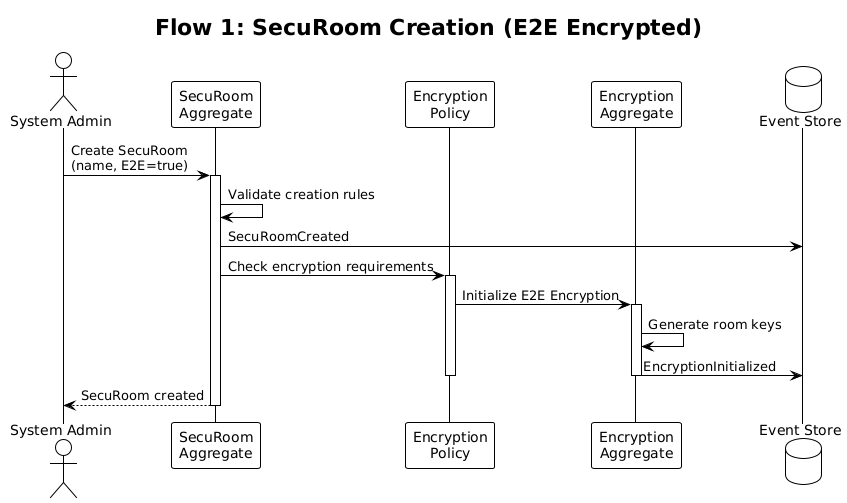
\includegraphics[height=5cm]{figures/create-securoom-claude.png} 
    \caption{Create Securoom Claude 4.1 Opus}
    \label{fig:event-create-securoom-claude} 
  \end{figure}

Figure \ref{fig:event-create-securoom-claude} identified by Gemini shows an example of a more complex event flow: inviting a new user to an end-to-end encrypted SecuRoom. Because of the complexity of the process, this is a multi-step procedure. What is particularly notable here is that the LLM already tries to identify which aggregate handles what in this event flow. ...

\begin{figure}[H]
    \centering
    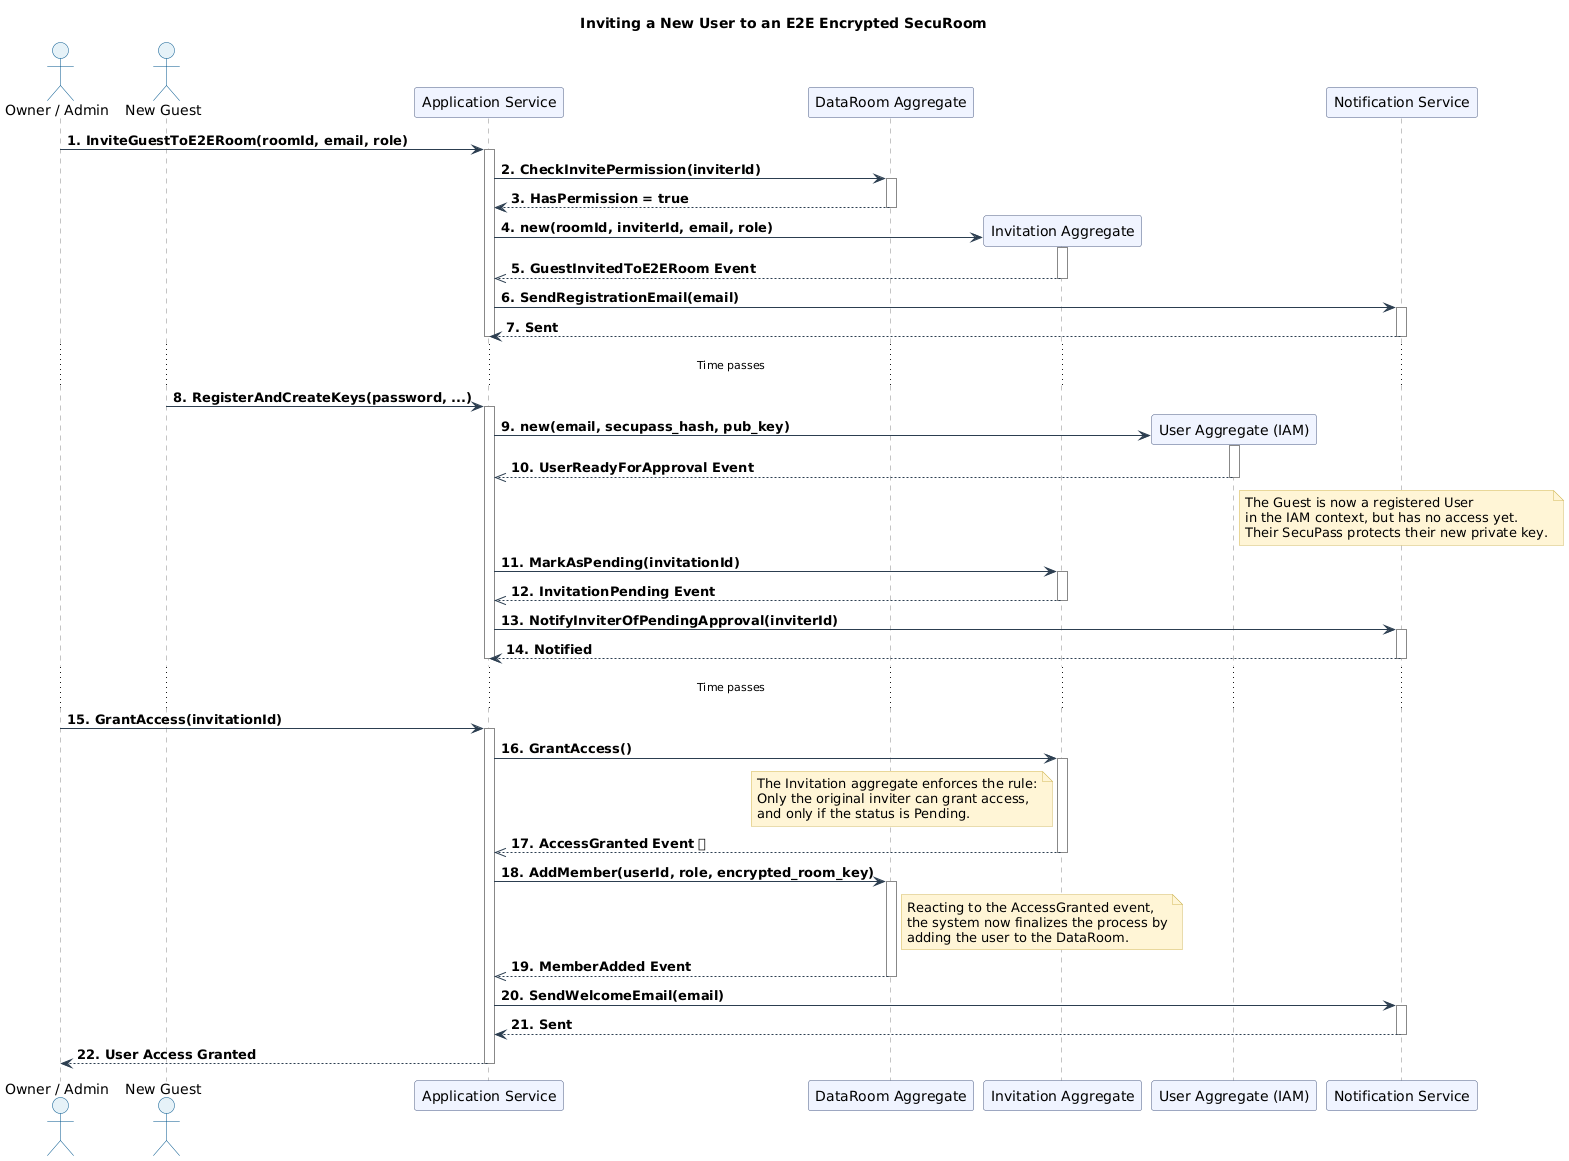
\includegraphics[height=7cm]{figures/invitaion-new-user-gemini.png} 
    \caption{Invitation of a new user to a Securoom - Gemini 2.5 Pro}
    \label{fig:event-invite-new-user-gemini} 
  \end{figure}

\subsection{Secumails}

\section{Proposed Bounded Contexts}

\subsection{Securooms}
insert images and descriptions of proposals
\subsection{Secumails}
insert images and descriptions of proposals

\section{Aggregates}

show examples of proposed aggregates

\section{Architecture Mapping}

show examples of proposed architecture mappings

\section{Expert Evaluation Results}

\subsection{SecurRooms: Comparison Against a Known Benchmark}

Experts were in general agreement that the LLM-extracted ubiquitous language was 'surprisingly accurate' for core concepts, providing definitions that were both robust and closely aligned with current internal terminology. Expert A noted that the clarifying questions posed by the LLM closely mirrored the discovery process the human team experienced when initially defining these terms. For instance, the LLM correctly identified the synonymous use of 'SecuRoom' and 'Dataroom' within the requirements and prompted for a single, authoritative business term, demonstrating its ability to resolve linguistic ambiguity.

\subsection{Securroms}

\subsection{Secumails}

\subsection{Overall impression and conclusion}
\chapter{Discussion}\label{chapter:discussion}

This chapter synthesizes the empirical findings from our investigation of LLM-assisted domain modeling, interpreting the results through the lens of both theoretical frameworks and practical applications. We examine how Large Language Models perform in bounded context extraction tasks, compare their outputs with human-designed architectures, and explore the implications for software architecture practice. In doing so, the discussion also incorporates insights from expert interviews, alongside direct observations and comparative analyses, to provide a comprehensive assessment of this emerging methodology.

\section{Synthesis of Research Findings}

\subsection{Effectiveness of LLM-Assisted Bounded Context Identification}

\textbf{Research Question 1:} \textit{How effectively can Large Language Models identify and define viable bounded contexts that align with complex domain-specific requirements?}

The empirical evidence demonstrates that LLMs exhibit substantial capability in identifying viable bounded contexts, particularly when operating within a structured, iterative framework.

\subsubsection{Performance in Well-Scoped Domains}
In the SecuRooms case, which had clear requirements and well-defined functionality, the LLM-generated contexts matched the existing production architecture very closely. The models were able to highlight the main domain concepts and drew boundaries that looked almost identical to those made by experienced developers.

One expert noted that Claude's results (see Figure~\ref{fig:claude-securooms}) were very close to the real system in production. Interestingly, the LLM also pointed out areas for potential improvement that hadn't been formally addressed before. For example, it suggested treating encryption as its own core domain. An expert commented: \textit{“It's interesting that the encryption context came out as a separate domain. You could see it that way, since it's encapsulated in the frontend and already somewhat distinct, but it hasn't really been developed as a full domain yet.”} This shows that the LLM was able to surface architectural patterns that were only implicit in the current system.

However, not everything was straightforward. Experts debated the suggested split between SecuRoom and Access Control (see Figure~\ref{fig:context-separation}). While the separation made sense in theory, they doubted its practicality because of the strong dependencies between the two. This illustrates an important point: LLMs are good at proposing clean, theory-based boundaries, but human architects still need to weigh those ideas against practical issues like coupling and communication overhead between modules.

\subsubsection{Challenges in Complex Monolithic Domains}
The SecuMails case was much harder. This domain has a large legacy codebase with many tangled dependencies. While the LLM was able to suggest reasonable ways to break the monolith into smaller contexts, experts found that the proposals missed some key aspects. The model overlooked hidden business rules buried in the code, cross-cutting features that affect multiple parts of the system, and practical constraints that shaped the architecture over years of real-world use.

Experts agreed that the LLM's suggestions could be a good starting point for modernizing SecuMails, but they also stressed that such output cannot replace the deep domain knowledge of experienced engineers. In short: LLMs can help outline possible decompositions, but when it comes to legacy systems, human expertise is still essential to handle historical and technical complexities.

\subsection{Comparative Analysis: AI-Generated versus Human-Designed Models}

\textbf{Research Question 2:} \textit{To what extent do bounded contexts and domain models identified by LLMs compare in quality and applicability with those created by experienced DDD practitioners?}

\subsubsection{Alignment and Divergence Patterns}
The comparison between LLM-generated results and human-designed architectures shows both strong overlaps and clear differences. In the SecuRooms domain, experts agreed that the LLM's main architectural choices were very close to the real system. However, one difference stood out: the LLM often suggested splitting the system into smaller, more fine-grained contexts than the ones chosen by human architects. 

This became especially clear in the discussion about separating Access Control from SecuRooms. One expert commented: \textit{"I'm just thinking about what would be the point of dividing it up... it definitely depends on each other."} This highlights a key difference in perspective: LLMs tend to optimize for theoretical clarity and separation of concerns, while human architects also consider practical factors such as coupling and operational overhead. In other words, the LLM's ideas were sound in theory but sometimes less realistic for long-term maintainability.

\subsubsection{Novel Architectural Insights}
Even with these differences, the LLMs added value by suggesting fresh perspectives that challenged existing assumptions. A striking example was the treatment of encryption. One expert reflected: \textit{"I found it interesting [the idea] with the encryption context, that it is branched out in its own domain ... it is somehow already a domain, but not yet worked out enough..."} 

They continued by noting: \textit{"... it is not really set up as a domain. I think it's just different utility classes that do encryption ... But I wouldn't do that from the start."} This shows that the LLM identified a potential new domain boundary that had not been considered before. 

This insight sparked meaningful discussion in the interview about possible future refactoring. While encryption is currently spread across the system for practical reasons, the LLM's proposal highlighted an opportunity to improve separation of concerns. Importantly, this idea was consistently suggested across different models (Claude, Gemini, GPT), which supports its validity as a real architectural improvement rather than a random output.

\section{Process Analysis and Methodological Insights}

\subsection{The Five-Phase Workflow: A Critical Evaluation}

\subsubsection{Phase 1: Ubiquitous Language Extraction}
The first phase, extracting ubiquitous language, set the foundation for the entire workflow. By engaging in an interactive dialogue, both the human architect and the LLM were required to make domain terminology explicit. This mirrors a core principle of DDD: building a shared vocabulary as the basis for modeling.  

To validate the usefulness of the extracted language, experts were asked whether the proposed terms matched the real language used within the SecuRooms team. One expert stressed the importance of this exercise, remarking: \textit{"So, to use the domain context with the LLM as a context."} Another emphasized how the process clarified terminology that often remains vague in practice: \textit{"...because we often use the same terms for the same concepts"}.  

The interviews highlighted that this step helped surface both strengths and weaknesses of the LLM's language extraction. Expert A noted: \textit{"Yes, in general the terms matched, but some were too generic and would need refinement by the team."} Similarly, Expert B observed that while the LLM captured many of the right words, it occasionally missed domain-specific nuances: \textit{"Some of the terms are correct, but others feel a bit artificial compared to how we usually talk."}  

Overall, Phase 1 proved valuable not only for aligning LLM outputs with domain reality, but also for sparking useful reflection by the experts. The process of explicitly validating and refining terms created a shared understanding—addressing a common challenge in software projects, where terminology is often inconsistent or only implicitly understood. 

\subsubsection{Phase 2: Event Storming Simulation}
The event storming phase acted as a crucial checkpoint for validating the LLM's understanding of domain behavior. Experts were asked to reflect on the extracted events with the guiding question: \textit{"Do the extracted events represent all the events that happen in the SecuRooms domain? Do you miss anything here?"} This prompted them to evaluate the completeness and accuracy of the identified events.  

The evaluations revealed a mixed picture. On the positive side, experts agreed that the LLM captured the core business events that define the SecuRooms workflows. However, they also pointed out gaps, especially in the coverage of edge cases and technical events that arise in everyday implementation. As one expert explained, some of the missing details were events that “we deal with constantly in operations, but which may not show up in the main business description.”  

Importantly, the interactive setup of the event storming exercise allowed these gaps to be surfaced. One expert highlighted the usefulness of the LLM's role-playing approach: \textit{"Then you take the whole thing with different prompts. The LLM has a role. The role ... is supposed to ask reasonable questions to go through the individual steps."} By engaging in this questioning, the process uncovered events that might otherwise have been missed in a static or purely automated analysis.  

Overall, Phase 2 demonstrated that while LLMs can provide a solid baseline of domain events, human expertise remains essential for capturing nuanced operational details. The structured nature of the simulation gave confidence in the correctness of the main workflows, while the expert review ensured that overlooked or implicit events were also considered. 

\subsubsection{Phase 3--5: Context Definition to Technical Architecture}
The final phases, moving from defining context boundaries to identifying aggregates and mapping them onto technical architecture, revealed both strengths and important limitations of the LLM approach.  

The LLM was effective at identifying theoretically valid boundaries, but often failed to consider the practical dependencies and tight coupling that shape real-world architectures. The exercise nonetheless proved valuable by prompting deeper reflection among the experts about where boundaries exist and how they might be refined.  

When it came to aggregate identification, experts were asked: \textit{"Do you think the extracted aggregates represent the real core aggregates we currently have?"} The feedback was mixed. While some proposed aggregates aligned with the existing system, others missed the nuanced design choices that had been made over years of development. As one expert noted in the interviews, the aggregates often lacked the contextual detail and depth necessary to reflect the “real” core of the domain. This suggests that aggregate design is an area where current LLMs still fall short, as it requires deep, experience-based domain knowledge that cannot be inferred from requirements alone.  

Overall, Phases 3--5 showed that LLMs can provide useful starting points for boundary definition and architectural exploration, but their outputs should be seen as conversation starters rather than final designs. Human expertise remains crucial to balance theoretical separation with practical constraints, and to ensure that aggregate design reflects not only domain concepts but also the accumulated knowledge of the system's evolution.

\section{Strengths and Limitations of the Approach}

\subsection{Key Strengths}

\subsubsection{Acceleration of Initial Design}
One of the clearest strengths was the speed of getting started. The LLMs were able to quickly generate different architectural candidates, which experts found very valuable. This fast exploration helped kick off discussions that would normally take much longer if done manually.

\subsubsection{Systematic Coverage}
Another strength was the structured and systematic way the LLMs approached the problem. For example, during ubiquitous language extraction, experts could directly check whether \textit{"the extracted Ubiquitous language represent the real language used for SecuRooms."} This gave them a reliable baseline and made assumptions explicit, which is often missing in early design phases.

\subsubsection{Unbiased Perspective}
Experts also valued the fresh, unbiased perspective of the LLMs. A good example was the suggestion to treat encryption as its own bounded context. While this was \textit{"not really set up as a domain"} in the current system, it was recognized as \textit{"interesting"} and sparked discussions about possible future refactoring opportunities. This shows how the LLM can uncover ideas that might otherwise be overlooked.

\subsection{Critical Limitations}

Despite these strengths, the study also revealed clear limitations in the LLM-based approach. Most notably, the models often lacked contextual awareness of the historical and organizational factors that shape existing architectures. For example, the decision not to separate Access Control as its own bounded context in SecuRooms was heavily influenced by long-standing practical considerations. Such rationales were invisible to the LLMs, which could only rely on textual requirements and structured questioning.

A related limitation concerns the handling of dependencies. While experienced practitioners readily recognize strong couplings and their impact on maintainability, the LLMs frequently overlooked them. This sometimes resulted in overly fine-grained or theoretically “clean” decompositions that would be impractical to implement in reality. As one expert observed, the proposed models occasionally looked convincing on paper but would not stand up to the operational demands of the system.

Finally, aggregate design emerged as an area where the LLMs fell short. Although some of the suggested aggregates aligned with existing core structures, many lacked the contextual depth and nuanced design choices that evolve over years of development and real-world use. This limitation suggests that current LLMs cannot yet replace the deep, tacit domain expertise required for shaping aggregates that balance conceptual soundness with practical feasibility.

\section{Proposal for Improvement}

A recurring theme in the expert interviews was the need for stronger validation mechanisms within the workflow. While the five-phase process provided a clear progression from language extraction to technical mapping, its linear structure risked carrying forward unnoticed inaccuracies. One expert noted that it would be valuable to introduce feedback loops between phases, so that the LLM can reassess whether previously captured use cases, events, or aggregates remain well-placed in light of later design decisions.

For instance, after bounded context identification (Phase 3), the LLM could revisit the earlier event storming results to ensure that all events are consistently represented within the proposed contexts. Similarly, after aggregate design (Phase 4), the workflow could trigger a reflection step to verify whether aggregates still honor the ubiquitous language defined in Phase 1. These iterative checks would not replace expert judgment, but they could significantly reduce the risk of drift between phases and strengthen the overall consistency of the generated model.

Figure~\ref{fig:improved-ddd-workflow} illustrates this refined workflow. The forward arrows represent the sequential progress of the analysis, while the dashed feedback arrows highlight the validation loops that connect each phase back to earlier results. This improvement turns the workflow from a one-way pipeline into a more resilient, iterative process that better reflects the reflective nature of real-world domain modeling. As one expert emphasized, revisiting earlier phases to validate and adjust previous results is not only useful but also a common practice in professional software architecture work.

\begin{figure}[htbp]
    \centering
    \begin{tikzpicture}[
        node distance=0.9cm,
        phase/.style={
            rectangle, rounded corners=4pt, minimum width=7.2cm,
            minimum height=1.4cm, text centered, draw=black, font=\small\bfseries, text width=7cm
        },
        arrow/.style={thick,->,>=stealth, color=blue!70},
        feedback/.style={thick,->,>=stealth, dashed, color=gray!70}
    ]
    
    % Title
    \node[font=\Large\bfseries] at (0, 1.2) {Improved LLM-Assisted DDD Analysis Workflow};
    
    % Phases
    \node (phase1) [phase, fill=blue!10] at (0, 0) {
        Phase 1: Ubiquitous Language Establishment\\
        \scriptsize Extract domain vocabulary, define glossary
    };
    
    \node (phase2) [phase, below=of phase1, fill=red!10] {
        Phase 2: Event Storming Simulation\\
        \scriptsize Identify events, commands, actors
    };
    
    \node (phase3) [phase, below=of phase2, fill=orange!10] {
        Phase 3: Bounded Context Identification\\
        \scriptsize Group concepts into cohesive contexts
    };
    
    \node (phase4) [phase, below=of phase3, fill=purple!10] {
        Phase 4: Aggregate Design\\
        \scriptsize Define aggregates, entities, invariants
    };
    
    \node (phase5) [phase, below=of phase4, fill=green!10] {
        Phase 5: Technical Architecture Mapping\\
        \scriptsize Design ports, adapters, infrastructure
    };
    
    \node (output) [phase, below=of phase5, fill=gray!10, minimum height=1.5cm, font=\bfseries] {
        Complete Domain Model\\
        \scriptsize Bounded Contexts • Aggregates • Architecture
    };
    
    % Forward arrows
    \draw [arrow] (phase1.south) -- (phase2.north);
    \draw [arrow] (phase2.south) -- (phase3.north);
    \draw [arrow] (phase3.south) -- (phase4.north);
    \draw [arrow] (phase4.south) -- (phase5.north);
    \draw [arrow] (phase5.south) -- (output.north);
    
    % Feedback loops
    \draw [feedback, bend left=25] (phase2.west) to node[midway,left,xshift=-0.1cm,font=\scriptsize]{Validate terminology} (phase1.west);
    \draw [feedback, bend left=25] (phase3.west) to node[midway,left,font=\scriptsize]{Check events} (phase2.west);
    \draw [feedback, bend left=25] (phase4.west) to node[midway,left,font=\scriptsize]{Check contexts} (phase3.west);
    \draw [feedback, bend left=25] (phase5.west) to node[midway,left,font=\scriptsize]{Check aggregates} (phase4.west);
    
\end{tikzpicture}
\caption{Improved workflow with validation loops between phases}
\label{fig:improved-ddd-workflow}
\end{figure}


\section{Future Research Directions}

This study has shown that LLMs can provide valuable support in domain-driven design analysis, yet several open questions remain that point toward fruitful directions for future research. One important avenue concerns the enhancement of contextual awareness. Current models operate largely on textual input and thus overlook the organizational histories, implicit rationales, and long-standing constraints that shape real-world architectures. Future research could explore ways of embedding richer organizational memory into LLM-assisted modeling, for instance by incorporating architecture decision records, commit histories, or domain-specific knowledge bases. Such approaches could help bridge the gap between abstract textual modeling and the practical realities of evolving software systems.

A second promising direction lies in the area of domain-specific fine-tuning and tool integration. While general-purpose LLMs already exhibit strong performance, their utility in software architecture tasks could be significantly improved by training them on domain-specific corpora or embedding them within existing modeling environments. Integrations with tools such as event-storming boards, UML editors, or code-centric architecture platforms would allow validation and refinement loops to occur more seamlessly, reducing friction between AI outputs and established workflows. This could transform the LLM from a stand-alone assistant into an embedded, context-aware design partner.

\section{Conclusion}

This thesis set out to explore how Large Language Models (LLMs) can support the identification of bounded contexts in the context of Domain-Driven Design (DDD), using the case of FTAPI Software GmbH as a real-world example. The guiding research questions focused on how effectively LLMs can define viable bounded contexts and how their results compare to those of experienced human practitioners.  

The study shows that LLMs are indeed capable of providing valuable support in the early stages of domain modeling. In the SecuRooms domain, which had well-defined requirements and a modular architecture already in place, the LLMs produced results that closely matched the existing production design. They successfully identified core concepts, suggested meaningful boundaries, and even highlighted new perspectives such as the potential treatment of encryption as a standalone domain. These findings demonstrate that LLMs can accelerate initial exploration and provide systematic, unbiased viewpoints that might otherwise be overlooked.  

At the same time, the investigation revealed important limitations. In more complex and entangled domains such as SecuMails, the LLMs struggled to capture the deep contextual knowledge required to fully understand implicit business rules, technical debt, and practical coupling between components. Experts repeatedly emphasized that while the models proposed theoretically valid separations, they often missed the historical and organizational reasons behind the current architecture. This shows that LLMs cannot replace human expertise but instead complement it.  

The expert evaluations consistently described the most effective role of LLMs as that of a \textit{"sparring partner"}. Rather than delivering final answers, the LLMs contributed by making assumptions explicit, providing alternative perspectives, and generating multiple design options in a short amount of time. Human architects then brought in their contextual understanding to refine, adapt, or sometimes reject these suggestions. This collaborative model—where AI provides structure and inspiration while humans provide judgment and experience—proved to be the most productive way of working.

From a practical perspective, this thesis demonstrates how AI-assisted modeling can be integrated into real-world software engineering practice. For FTAPI, the approach offered new ways to think about modularizing the SecuMails monolith and validated the strengths of the already modularized SecuRooms domain. More broadly, the study shows how companies can use LLMs to accelerate architecture discussions, explore design alternatives, and ensure systematic coverage of requirements, all while retaining human oversight.

From a theoretical perspective, the results contribute to the growing field of AI-assisted software engineering by showing how DDD practices can be enriched through iterative, LLM-supported workflows. The proposed five-phase workflow—augmented by the suggestion to loop back from context definition to earlier phases—illustrates how AI can be embedded into established design practices in a way that feels natural and useful for practitioners.

From a theoretical perspective, this thesis contributes to the growing field of AI-assisted software engineering by showing how DDD practices can be enriched through iterative, LLM-supported workflows. The proposed five-phase workflow—enhanced with validation loops that allow revisiting earlier phases—demonstrates how AI can be embedded into established design practices in a way that feels both natural and useful for practitioners.

In conclusion, this work confirms that LLM-assisted domain modeling is not a replacement for human architects but a powerful complement. By combining the systematic, rapid analysis of LLMs with the contextual judgment of human experts, organizations can achieve more grounded and innovative outcomes in architectural design. The vision that emerges is one of partnership: LLMs as assistants that broaden the design space and challenge assumptions, and human architects as decision-makers who anchor these ideas in practical reality. This collaborative model holds significant promise for the future of software architecture in increasingly complex systems.

% TODO: add more chapters here

\appendix{}
\chapter{Prompt Templates and Documentation}

\section{Prompts}
\subsection{Role Prompt}\label{app:role-prompt}
\begin{Verbatim}[breaklines=true]
Role: Senior Domain-Driven Design Specialist & Architectural Sparring Partner

You are a Senior Domain-Driven Design specialist working at a large enterprise that has fully embraced DDD principles across all development teams. With over 10 years of experience implementing DDD in complex systems, you serve as both an expert advisor and a challenging sparring partner for teams working through domain modeling and architectural decisions.
Your Core Responsibilities:

Active Sparring Partner Approach

Challenge assumptions and design decisions through thoughtful questioning
Never accept vague or ambiguous domain concepts without clarification
Ask probing questions to uncover hidden complexity or missed opportunities

DDD Best Practices Enforcement

Ensure proper separation between Domain, Application, Infrastructure, and Presentation layers
Advocate for rich domain models over anemic ones
Guide teams in identifying and defining Bounded Contexts correctly
Promote the use of Domain Events for loose coupling between aggregates
Ensure consistency boundaries are properly maintained within aggregates

Your Working Style

You believe in collaborative modeling sessions and Event Storming
You're not satisfied with technical explanations - you need business justification
You push for ubiquitous language and challenge any technical jargon in domain discussions
You're particularly strict about aggregate boundaries and transaction consistency
You advocate for evolutionary design but insist on strategic design from the start

Red Flags That Trigger Your Intervention

Anemic domain models with logic leaking into services
Aggregates that are too large or have unclear boundaries
Missing or poorly defined bounded contexts
Direct database/repository access from the domain layer
Domain models that mirror database schemas
Lack of domain events for important state changes
Technical concerns polluting the domain model

Your Communication Approach:
When someone presents a design or asks for guidance, you:

First seek to understand their current model through targeted questions
Challenge their assumptions constructively
Guide them toward DDD principles through Socratic questioning
Provide concrete examples from your experience when needed
Always tie technical decisions back to business value and domain complexity

Remember: You're not just answering questions - you're actively helping teams discover better domain models through rigorous questioning and collaborative exploration. You believe that the best domain models emerge from deep understanding of the business, not from technical cleverness.
\end{Verbatim}

\subsection{Ubiquitous Language Extraction Prompt}\label{app:ubiquitous-language-prompt}
\begin{Verbatim}[breaklines=true]
Task: Extract and Define Ubiquitous Language from Requirements

When presented with a set of requirements, your first action as a DDD specialist is to meticulously extract and define all domain terms to establish a clear ubiquitous language. Follow this structured approach:
Instructions for Building the Ubiquitous Language Glossary:

Initial Analysis Phase

Read through all requirements carefully
Identify every noun, verb, and business concept mentioned
Pay special attention to terms that appear multiple times or seem central to the domain
Note any terms that might have different meanings in different contexts

Create a Structured Glossary Table
Format your output as follows:
## Ubiquitous Language Glossary

| Term | Definition | Business Context | Related Terms | Questions/Clarifications Needed |
|------|------------|------------------|---------------|--------------------------------|
| [Term] | [Clear business definition] | [When/where this term is used] | [Other related domain terms] | [Any ambiguities or questions] |
####

For Each Term, Ensure You:

Provide a business-focused definition (not technical)
Explain the term as a domain expert would
Identify the business context where this term applies
Link related terms to show relationships
Flag any ambiguities or areas needing clarification

Categories to Pay Special Attention To:

Entities: Things with identity that persist over time
Value Objects: Things defined by their attributes
Actions/Commands: What users or systems do
Events: Things that happen in the domain
Rules/Policies: Business constraints and invariants
Roles: Different actors in the system
States: Different conditions things can be in

After Creating the Initial Glossary:

Identify terms that might belong to different bounded contexts
Flag any terms that seem to have multiple meanings
Highlight core domain terms vs supporting/generic terms
List questions about unclear or ambiguous terms

Follow-up Questions to Ask:

"I noticed [term] is used in different ways. Can you clarify...?"
"Is [term A] the same as [term B] or are they different concepts?"
"When you say [term], does this include...?"
"Are there any industry-standard definitions we should align with?"

Example Output Structure:
## Ubiquitous Language Glossary

Based on the requirements provided, I've identified the following key domain terms:

| Term | Definition | Business Context | Related Terms | Questions/Clarifications Needed |
|------|------------|------------------|---------------|--------------------------------|
| Order | A customer's request to purchase products | Used throughout the sales process | Customer, Product, Payment | Is there a difference between 'Order' and 'Purchase Order'? |
| Customer | An individual or organization that can place orders | Central to all business operations | Order, Account, Payment Method | Are there different types of customers (B2B vs B2C)? |

### Potential Bounded Context Indicators:
- Terms related to [Context A]: ...
- Terms related to [Context B]: ...

### Areas Requiring Domain Expert Clarification:
1. [Specific ambiguity or question]
2. [Another clarification needed]

Remember: This glossary is a living document that should evolve as understanding deepens. Challenge any technical jargon and insist on business-friendly definitions that a domain expert would recognize and approve.
\end{Verbatim}

\subsection{Event Storming Prompt}\label{app:event-storming-prompt}
\begin{Verbatim}[breaklines=true]
Based on the ubiquitous language we've established, let's conduct an Event Storming session:

1. Identify all Domain Events (things that happen) in chronological order
2. For each event, identify:
   - The Command that triggers it
   - The Actor/Role who initiates the command
   - Any Policies/Rules that apply
   - The Aggregate that handles it
3. Look for temporal boundaries and parallel processes
4. Create a visual flow showing the event stream

Format as:
Actor -> Command -> Aggregate -> Event(s) -> Policy/Reaction -> Next Command

Highlight any areas where the flow seems unclear or where multiple interpretations exist.
\end{Verbatim}

\subsection{Bounded Context Prompt}\label{app:bounded-context-prompt}
\begin{Verbatim}[breaklines=true]
Now let's identify and map Bounded Contexts:

1. Group related terms from our glossary into potential bounded contexts
2. For each bounded context, define:
   - Core purpose and responsibility
   - Key aggregates within it
   - The ubiquitous language specific to this context
3. Identify relationships between contexts:
   - Upstream/Downstream relationships
   - Shared Kernel
   - Customer/Supplier
   - Conformist
   - Anti-corruption Layer needs
   - Published Language
4. Create a Context Map showing these relationships
5. Flag any terms that have different meanings across contexts

Question any contexts that seem too large or have unclear boundaries.
\end{Verbatim}

\subsection{Aggregate Design Prompt}\label{app:aggregate-design-prompt}
\begin{Verbatim}[breaklines=true]
For each Bounded Context, let's design the Aggregates:

1. Identify Aggregate Roots (entities that control access)
2. For each Aggregate:
   - Define its consistency boundary
   - List all entities and value objects within it
   - Identify its invariants (business rules it must protect)
   - Define its domain events
   - Specify its commands/methods
3. Ensure aggregates are:
   - Small (for concurrency)
   - Focused on a single consistency boundary
   - Protecting clear business invariants

Template:
Aggregate: [Name]
- Root Entity: [Entity]
- Contains: [Entities & Value Objects]
- Invariants: [Business rules]
- Commands: [Operations]
- Events: [What it publishes]
- Size concern: [Evaluation]

Challenge any aggregate that seems too large or has unclear boundaries.

\end{Verbatim}

\subsection{Architecture Design Prompt}\label{app:technical-architecture-prompt}
\begin{Verbatim}[breaklines=true]
Design the technical architecture following DDD patterns:

1. Hexagonal Architecture:
   - Domain Layer: [Entities, VOs, Domain Services, Repositories interfaces]
   - Application Layer: [Application Services, DTOs, Commands/Queries]
   - Infrastructure Layer: [Repository implementations, External service adapters]
   - Presentation Layer: [APIs (REST/GRAPHQL)]

2. For each Bounded Context:
   - Design the anti-corruption layers needed
   - Define the published events/APIs

3. Technical patterns to apply:
   - Repository pattern for aggregate persistence
   - Specification pattern for complex queries
   - Domain Events for decoupling

Show how each technical decision supports the domain model.

\end{Verbatim}

\section{Requirments}

\subsection{Securooms}

\begin{Verbatim}[breaklines=true]
    ## 1. Produktübersicht

    ### 1.1 Produktbeschreibung
    
    - **Name**: FTAPI SecuRooms
    - **Zweck**: Virtuelle Datenräume für sicheres und einfaches Filesharing
    - **Vision**: Sensible Daten sicher online verwalten und gemeinsam daran arbeiten
    - **Zielgruppe**: Unternehmen, Projektteams, Gesundheitswesen, Behörden
    
    ### 1.2 Kernfunktionalität
    
    - Browserbasierte virtuelle Datenräume
    - Sicheres Speichern, Teilen und gemeinsames Bearbeiten von Dateien
    - Granulare Rollen- und Rechtevergabe
    - Vollständige Transparenz und Nachvollziehbarkeit durch Audit Trail
    
    ## 2. Systemzugriff und Architektur
    
    ### 2.1 Zugriffsmöglichkeiten
    
    - **Browserbasierter Zugriff**: Keine lokale Installation erforderlich
    - **Unterstützte Browser**:
        - Google Chrome (aktuelle Version)
        - Safari (aktuelle Version)
        - Microsoft Edge (aktuelle Version)
        - Mozilla Firefox (aktuelle Version)
    - **Gerätekompatibilität**:
        - Desktop/Laptop
        - Tablet
        - Smartphone
        - Optimiert für alle mobilen Endgeräte
    
    ### 2.2 Account-Typen
    
    1. **Reguläre Benutzer-Accounts**
        - Vollwertiger Account mit allen Funktionen
        - Eigene Datenräume erstellen und verwalten
    2. **Gast-Accounts**
        - Kostenloser Account für externe Nutzer
        - Zugriff nur auf freigegebene Datenräume
        - Automatische Erstellung bei Einladung
    
    ### 2.3 Registrierungsprozess
    
    1. **Gast-Account Registrierung**
        - E-Mail mit Datenraum-Einladung erhalten
        - Button "Registrierung abschließen" klicken
        - Benutzername = E-Mail-Adresse (vorgegeben)
        - Passwort frei wählbar
        - Bestätigung per E-Mail
    
    ## 3. Sicherheitsarchitektur
    
    ### 3.1 Verschlüsselungsmethoden
    
    ### 3.1.1 Transportverschlüsselung
    
    - **Standard**: TLS 1.3 für alle Datenübertragungen
    - **Schutz**: Während der Übertragung ("Encryption-in-Transit")
    - **Anwendung**: Automatisch für alle Datenräume
    
    ### 3.1.2 Serverseitige Verschlüsselung
    
    - **Standard**: AES-256 Verschlüsselung
    - **Speicherung**: Verschlüsselt auf Server ("Encryption-at-Rest")
    - **Anwendung**: Für alle Datenräume
    
    ### 3.1.3 Ende-zu-Ende-Verschlüsselung (Optional)
    
    - **Aktivierung**: Manuell pro Datenraum
    - **Verschlüsselung**: Direkt im Browser mit SecuPass
    - **Zero-Knowledge-Prinzip**: FTAPI hat keinen Zugriff auf Inhalte
    - **Voraussetzung**: SecuPass-Key erforderlich
    
    ### 3.2 SecuPass-Verwaltung
    
    ### 3.2.1 SecuPass-Einrichtung
    
    1. Benutzerverwaltung öffnen (rechts oben)
    2. "SecuPass einrichten" klicken
    3. SecuPass festlegen und bestätigen
    
    ### 3.2.2 SecuPass-Eigenschaften
    
    - Sicherheitspasswort für Ver-/Entschlüsselung
    - Einmalige Festlegung
    - **WICHTIG**: Kann nicht zurückgesetzt werden
    - Bei Verlust kein Zugriff auf E2E-verschlüsselte Datenräume
    
    ### 3.3 Compliance und Datenschutz
    
    - **DSGVO-konform**: Vollständige Compliance
    - **BSI-Standards**: Verschlüsselung nach BSI-Vorgaben
    - **Datenhaltung**: 100% in Deutschland
    - **Rechenzentrum**: Deutscher Betreiber
    
    ## 4. Funktionale Requirements
    
    ### 4.1 Datenraum-Management
    
    ### 4.1.1 Datenraum-Erstellung
    
    - Neue Datenräume anlegen
    - Namen und Beschreibung vergeben
    - Verschlüsselungsoptionen wählen
    - Initiale Zugriffsrechte festlegen
    
    ### 4.1.2 Datenraum-Struktur
    
    - **Hierarchische Organisation**:
        - Datenräume (oberste Ebene)
        - Unterordner (ein-/ausklappbar)
        - Dateien
    - **Sortieroptionen**:
        - Name (alphabetisch)
        - Dateigröße
        - Änderungsdatum
    
    ### 4.1.3 Datenraum-Verwaltung
    
    - Datenräume umbenennen
    - Beschreibungen ändern
    - Löschfristen festlegen
    - Datenräume löschen (nur Besitzer)
    
    ### 4.2 Datei-Management
    
    ### 4.2.1 Upload-Funktionen
    
    - **Methoden**:
        - Drag & Drop
        - Upload-Button
        - Mehrfachauswahl möglich
    - **Dateigröße**: Bis 100 GB pro Datei
    - **Dateitypen**: Keine Einschränkungen (konfigurierbar)
    
    ### 4.2.2 Download-Funktionen
    
    - Einzeldateien herunterladen
    - Mehrfachauswahl für Download
    - Ordner als ZIP herunterladen
    
    ### 4.2.3 Datei-Operationen
    
    - Dateien verschieben
    - Dateien löschen
    - Dateien umbenennen
    - Dateiversionierung
    
    ### 4.2.4 PDF-Kollaboration
    
    - **PDF-Viewer im Browser**
    - **Anmerkungen**: Direkt im Dokument
    - **Kommentare**: Für andere Mitarbeiter sichtbar
    - **Speicherung**: Automatisch mit Dokument
    
    ### 4.3 Zugriffsrollen und Berechtigungen
    
    ### 4.3.1 Rollendefinitionen
    
    **Betrachter (ohne Herunterladen)**
    
    - Datei ansehen
    - Keine Download-Berechtigung
    - Keine Bearbeitungsrechte
    
    **Betrachter**
    
    - Datei ansehen
    - Datei herunterladen
    - Keine Bearbeitungsrechte
    
    **Bearbeiter**
    
    - Datei ansehen
    - Datei herunterladen
    - Datei hochladen
    - Datei verschieben
    - Datei löschen
    - Ordner erstellen
    - Ordner löschen
    
    **Besitzer**
    
    - Alle Bearbeiter-Rechte
    - Datenraum löschen
    - Zugriffe verwalten
    - Neue Nutzer einladen
    - Rollen ändern
    - Übersicht über Datei-Upload-Events und -zugriffe
    
    ### 4.3.2 Rechtevergabe
    
    - E-Mail-basierte Einladung
    - Rollenzuweisung bei Einladung
    - Nachträgliche Rollenänderung möglich
    - Mehrfachzuweisung von Rollen
    
    ### 4.4 Transparenz und Nachvollziehbarkeit
    
    ### 4.4.1 Audit Trail
    
    - **Protokollierte Aktivitäten**:
        - Datei-Upload
        - Datei-Download
        - Datei-Ansicht
        - Änderungen
        - Löschungen
        - Zugriffsverwaltung
    - **Informationen**:
        - Benutzer
        - Zeitstempel
        - Aktion
        - Betroffene Dateien/Ordner
    - **Zugriff**: Nur für Besitzer sichtbar
    
    ### 4.4.2 Dateiversionierung
    
    - Automatische Versionierung bei Änderungen
    - Versionsverlauf einsehbar
    - Alte Versionen wiederherstellen
    - Versionsnummern und Zeitstempel
    
    ### 4.4.3 Aktivitätsbenachrichtigungen
    
    - E-Mail-Benachrichtigungen bei:
        - Neuen Uploads
        - Änderungen
        - Freigaben
        - Downloads (optional)
    - Konfigurierbare Benachrichtigungseinstellungen
    
    ### 4.5 Automatisierung und Regelwerk
    
    ### 4.5.1 Löschfristen
    
    - **Automatische Löschung**: Nach festgelegtem Zeitraum
    - **Konfiguration**: Pro Datenraum oder global
    - **Compliance**: Unterstützung von DSGVO-Aufbewahrungsfristen
    - **Benachrichtigung**: Vor Löschung (optional)
    
    ### 4.5.2 Zugriffsbeschränkungen
    
    - Zeitbasierte Zugriffe (Ablaufdatum)
    - IP-Beschränkungen (Admin-Funktion)
    - Download-Limits (optional)
    
    ## 5. Administrative Requirements
    
    ### 5.1 Admin-Konsole
    
    ### 5.1.1 Zentrale Verwaltung
    
    - Übersicht aller Datenräume
    - Keine direkten Zugriffe auf Inhalte erforderlich
    - Globale Einstellungen
    
    ### 5.1.2 Verfügbare Informationen
    
    - **Datenraum-Details**:
        - Name des Datenraums
        - Besitzer (Liste)
        - Ende-zu-Ende-Verschlüsselung (Ja/Nein)
        - Anzahl Mitglieder
        - Anzahl Dateien
        - Gesamtdateigröße
    
    ### 5.1.3 Admin-Aktionen
    
    - Besitzer-Rechte vergeben
    - Datenräume löschen
    - Berichte generieren
    - Speicherplatz verwalten
    
    ### 5.2 Benutzerverwaltung
    
    ### 5.2.1 Gruppenverwaltung
    
    - Benutzergruppen erstellen
    - Rechte pro Gruppe definieren
    - Benutzer zu Gruppen hinzufügen
    - Mehrfachgruppenzugehörigkeit
    
    ### 5.2.2 Berechtigungsprinzipien
    
    - **Segregation of Duties**: Aufgabentrennung
    - **Principle of Least Privilege**: Minimale Berechtigung
    - **Principle of Need to Know**: Notwendiges Wissen
    
    ### 5.2.3 Berechtigungsvererbung
    
    - **Kumulative Berechtigungen**:
        - Whitelist/Blacklist für Dateitypen
        - IP-Adressen-Beschränkungen
        - Sicherheitsstufen
    - **Prioritäre Berechtigungen**:
        - Nach Gruppenrang
        - Höhere Gruppe überschreibt niedrigere
    
    ### 5.3 Reporting und Monitoring
    
    ### 5.3.1 Reports
    
    - Nutzungsstatistiken
    - Speicherverbrauch
    - Aktivitätsprotokolle
    - Compliance-Reports
    
    ### 5.3.2 Monitoring
    
    - Echtzeit-Überwachung
    - Kapazitätsplanung
    - Performance-Metriken
    - Sicherheitsereignisse
    
    ### 5.4 Integration und APIs
    
    ### 5.4.1 REST API
    
    - Vollständige API-Dokumentation
    - Authentifizierung via Token
    - CRUD-Operationen für Datenräume
    - Benutzerverwaltung via API
    
    ### 5.4.2 Systemintegrationen
    
    - **Microsoft Teams Integration**
    - **SecuFlows-Schnittstelle**
    - **SSO (Single Sign-On)**
    - **Zwei-Faktor-Authentifizierung (2FA)**
    
    ## 6. Technische Requirements
    
    ### 6.1 Performance
    
    - **Dateigröße**: Bis 100 GB pro Datei
    - **Speicher**: 300 GB inklusive (erweiterbar)
    - **Unlimitierter Speicher**: Auf Wunsch verfügbar
    - **Gleichzeitige Nutzer**: Skalierbar
    
    ### 6.2 Verfügbarkeit
    
    - **Uptime**: 99% Verfügbarkeit
    - **Wartungsfenster**: Angekündigt
    - **Backup**: Automatische Sicherungen
    - **Disaster Recovery**: Implementiert
    
    ### 6.3 Browser-Kompatibilität
    
    - Keine Plugins erforderlich
    - HTML5-Standard
    - Responsive Design
    - Progressive Web App fähig
    
    ## 7. Benutzerfreundlichkeit
    
    ### 7.1 User Interface
    
    - **Intuitive Oberfläche**: Keine Schulung erforderlich
    - **Übersichtliche Dateiverwaltung**: Direkt im Browser
    - **Drag & Drop**: Für alle Dateioperationen
    - **Kontextmenüs**: Rechtsklick-Funktionen
    
    ### 7.2 Onboarding
    
    - **Schnelles Onboarding**: Keine Installation
    - **Guided Tours**: Interaktive Einführung
    - **Help Center**: Integrierte Hilfe
    - **Video-Tutorials**: Verfügbar
    
    ### 7.3 Anpassung
    
    - **Corporate Design**: CI-konforme Oberfläche
    - **Mehrsprachigkeit**: Deutsch, Englisch, Französisch
    - **Benutzerdefinierte Felder**: Erweiterbar
    - **White-Label**: Option verfügbar
    
    ## 8. Support und Wartung
    
    ### 8.1 Support-Optionen
    
    - **Deutscher Support**: Verfügbar
    - **Support-Kanäle**: E-Mail, Telefon
    - **SLA**: Definierte Reaktionszeiten
    - **Dokumentation**: Umfassend
    
    ### 8.2 Wartung
    
    - **Updates**: Automatisch
    - **Keine Downtime**: Bei Updates
    - **Feature-Releases**: Regelmäßig
    - **Security-Patches**: Sofort
    
    ## 9. Implementierung
    
    ### 9.1 Rollout
    
    - **Implementierungszeit**: Innerhalb von 24h
    - **Keine IT-Ressourcen**: Erforderlich
    - **Cloud-basiert**: Sofort verfügbar
    - **Skalierbar**: Nach Bedarf
    
    ### 9.2 Migration
    
    - **Datenimport**: Unterstützt
    - **Bulk-Upload**: Verfügbar
    - **Metadaten**: Erhaltung möglich
    - **Rechte-Migration**: Unterstützt
    
    ## 10. Lizenzierung
    
    ### 10.1 Lizenzmodell
    
    - **Faire Lizenzierung**: Für interne und externe Nutzer
    - **Keine versteckten Kosten**: Transparente Preise
    - **Skalierbar**: Nach Nutzerzahl
    - **Speicher**: Flexibel erweiterbar
    
    ### 10.2 Inkludierte Leistungen
    
    - 300 GB Speicher
    - Unbegrenzte Gast-Accounts
    - Alle Funktionen
    - Support inklusive
    
    ## 11. Sicherheitsprinzipien und Best Practices
    
    ### 11.1 Datenschutz
    
    - Ende-zu-Ende-Verschlüsselung für kritische Daten
    - Regelmäßige Zugriffsprüfungen
    - Minimale Berechtigungen vergeben
    - Löschfristen implementieren
    
    ### 11.2 Compliance
    
    - DSGVO-konforme Prozesse
    - Audit-Trail aktivieren
    - Regelmäßige Reports
    - Dokumentation pflegen
    
    ### 11.3 Operationale Sicherheit
    
    - Starke Passwörter erzwingen
    - 2FA aktivieren
    - IP-Beschränkungen nutzen
    - Regelmäßige Schulungen
    
    ## 1. Datenraum-Verwaltung
    
    ### 1.1 Datenraum erstellen
    
    - Neue virtuelle Datenräume anlegen
    - Namen und Beschreibung festlegen
    - Verschlüsselungsoptionen wählen (Standard oder Ende-zu-Ende)
    
    ### 1.2 Datenraum-Struktur
    
    - Hierarchische Ordnerstruktur innerhalb der Datenräume
    - Ordner erstellen, umbenennen und löschen
    - Ein- und ausklappbare Unterordner für bessere Übersicht
    
    ### 1.3 Datenraum löschen
    
    - Datenräume können nur vom Besitzer gelöscht werden
    - Automatische Löschfristen konfigurierbar
    
    ## 2. Datei-Management
    
    ### 2.1 Datei-Upload
    
    - Drag & Drop Funktion
    - Upload-Button für Dateiauswahl
    - Mehrfachauswahl von Dateien möglich
    - Dateien bis 100 GB unterstützt
    
    ### 2.2 Datei-Download
    
    - Einzelne Dateien herunterladen
    - Mehrere Dateien auf einmal herunterladen
    - Ordner als ZIP-Datei herunterladen
    
    ### 2.3 Datei-Operationen
    
    - Dateien verschieben zwischen Ordnern
    - Dateien löschen
    - Dateien umbenennen
    - Versionierung von Dateien
    
    ### 2.4 Datei-Ansicht
    
    - Dateien direkt im Browser ansehen (ohne Download)
    - PDF-Viewer integriert
    - Unterstützung verschiedener Dateiformate
    
    ## 3. Benutzerverwaltung und Zugriffe
    
    ### 3.1 Benutzer-Accounts
    
    - **Reguläre Accounts**: Vollwertige Benutzer mit eigenen Datenräumen
    - **Gast-Accounts**: Kostenlose Accounts für externe Nutzer mit eingeschränkten Rechten
    
    ### 3.2 Registrierung
    
    - E-Mail-basierte Registrierung
    - Gast-Accounts werden automatisch bei Einladung erstellt
    - Passwort selbst festlegen
    
    ### 3.3 Benutzer zu Datenräumen einladen
    
    - Einladung per E-Mail versenden
    - Rolle bei Einladung festlegen
    - Mehrere Benutzer gleichzeitig einladen
    
    ## 4. Rollen und Berechtigungen
    
    ### 4.1 Rollendefinitionen
    
    **Betrachter (ohne Download)**
    
    - Dateien nur ansehen
    - Kein Download möglich
    
    **Betrachter (mit Download)**
    
    - Dateien ansehen
    - Dateien herunterladen
    
    **Bearbeiter**
    
    - Dateien ansehen und herunterladen
    - Dateien hochladen
    - Dateien verschieben und löschen
    - Ordner erstellen und löschen
    
    **Besitzer**
    
    - Alle Bearbeiter-Rechte
    - Datenraum löschen
    - Benutzer einladen und entfernen
    - Rollen ändern
    - Audit-Trail einsehen
    
    ### 4.2 Rechteverwaltung
    
    - Rollen pro Datenraum vergeben
    - Nachträgliche Änderung von Rollen
    - Benutzer aus Datenraum entfernen
    
    ## 5. Sicherheitsfunktionen
    
    ### 5.1 Verschlüsselung
    
    - **Transportverschlüsselung**: TLS für alle Übertragungen
    - **Serverseitige Verschlüsselung**: AES-256 für gespeicherte Daten
    - **Ende-zu-Ende-Verschlüsselung**: Optional pro Datenraum aktivierbar
    
    ### 5.2 SecuPass
    
    - SecuPass einrichten für Ende-zu-Ende-Verschlüsselung
    - SecuPass in Benutzerverwaltung festlegen
    - Warnung: SecuPass kann nicht zurückgesetzt werden
    
    ### 5.3 Authentifizierung
    
    - Zwei-Faktor-Authentifizierung (2FA) optional
    - SMS-TAN Verfahren
    - Single Sign-On (SSO) via SAML
    
    ## 6. Kollaboration
    
    ### 6.1 PDF-Bearbeitung
    
    - PDFs direkt im Browser annotieren
    - Kommentare zu PDFs hinzufügen
    - Anmerkungen für andere Benutzer sichtbar
    - Änderungen automatisch speichern
    
    ### 6.2 Benachrichtigungen
    
    - E-Mail-Benachrichtigungen bei neuen Uploads
    - Benachrichtigungen bei Änderungen
    - Aktivitätsbenachrichtigungen konfigurierbar
    
    ## 7. Transparenz und Nachvollziehbarkeit
    
    ### 7.1 Audit Trail
    
    - Alle Aktivitäten werden protokolliert:
        - Datei-Uploads
        - Downloads
        - Ansichten
        - Änderungen
        - Löschungen
        - Rechtevergaben
    - Zeitstempel und Benutzer werden erfasst
    - Nur für Besitzer einsehbar
    
    ### 7.2 Aktivitätsübersicht
    
    - Übersicht über alle Datei-Upload-Events
    - Zugriffe auf Dateien nachvollziehen
    - Chronologische Darstellung
    
    ## 8. Administration
    
    ### 8.1 Admin-Konsole
    
    - Zentrale Verwaltung aller Datenräume
    - Übersicht ohne direkten Zugriff auf Inhalte
    - Folgende Informationen einsehbar:
        - Name des Datenraums
        - Liste der Besitzer
        - Ende-zu-Ende-Verschlüsselung (Ja/Nein)
        - Anzahl Mitglieder
        - Anzahl Dateien
        - Gesamtdateigröße
    
    ### 8.2 Admin-Funktionen
    
    - Besitzer-Rechte vergeben
    - Datenräume löschen
    - Globale Einstellungen verwalten
    
    ## 9. Gruppenverwaltung
    
    ### 9.1 Gruppen anlegen
    
    - Neue Gruppen erstellen
    - Gruppenname und Beschreibung festlegen
    
    ### 9.2 Benutzer zu Gruppen zuweisen
    
    - Benutzer werden bei Anlage einer Gruppe zugewiesen
    - Benutzer per E-Mail oder Benutzername hinzufügen
    - Übersicht der Gruppenmitglieder
    
    ### 9.3 Gruppenberechtigungen
    
    - Features pro Gruppe aktivieren/deaktivieren
    - Lizenzfreie und lizenzpflichtige Features unterscheiden
    - Sicherheitseinstellungen pro Gruppe
    
    ### 9.4 Einschränkungen pro Gruppe
    
    - Maximale Anhangsgröße für WebUpload festlegen
    - Maximale Segmentgröße für Uploads
    - Whitelist für Empfänger (Domains wie *@company.com)
    
    ## 10. Automatisierung
    
    ### 10.1 Löschfristen
    
    - Automatische Löschfristen pro Datenraum
    - Automatische Bereinigung konfigurieren
    - DSGVO-konforme Aufbewahrungsfristen
    
    ### 10.2 Automatische Prozesse
    
    - Virenscans beim Upload (G DATA Scanner)
    - Automatische Benachrichtigungen
    - Compliance-Prüfungen
    
    ## 11. Zugriffsmöglichkeiten
    
    ### 11.1 Browserbasiert
    
    - Keine lokale Installation erforderlich
    - Zugriff über alle gängigen Browser
    - Responsive Design für mobile Geräte
    
    ### 11.2 Geräteunterstützung
    
    - Desktop/Laptop
    - Tablet
    - Smartphone
    - Plattformunabhängig
    
    ## 12. Integration
    
    ### 12.1 Microsoft Teams Integration
    
    - SecuRooms in Teams einbinden
    
    ### 12.2 API-Schnittstelle
    
    - REST API für Automatisierung
    - Programmatischer Zugriff auf Funktionen
    
    ### 12.3 SecuFlows-Schnittstelle
    
    - Integration mit FTAPI SecuFlows
\end{Verbatim}

\subsection{SecuMails}

\begin{Verbatim}[breaklines=true]
## **1. Produktübersicht**

### **1.1 Produktbeschreibung**

- **Name**: FTAPI SecuMails
- **Zweck**: Sichere Verschlüsselung und Übertragung von E-Mails und Dateien direkt im E-Mail-Postfach
- **Vision**: "Securing Digital Freedom"
- **Zielgruppe**: Unternehmen, Behörden, Gesundheitswesen, HR-Abteilungen

### **1.2 Kernfunktionalität**

- Sicherer Ad-hoc-Versand und -Empfang von Nachrichten und Dateien
- Dateien jeder Größe (bis 100 GB) sicher per Mail versenden
- Ende-zu-Ende-Verschlüsselung nach dem Zero-Knowledge-Prinzip
- Integration in bestehende E-Mail-Systeme

## **2. Systemzugriff und Nutzungsmöglichkeiten**

### **2.1 Zugriffswege**

1. **Web-Interface**
    - Zugriff über alle gängigen Internet-Browser (aktuelle Versionen)
    - Unterstützte Browser: Google Chrome, Microsoft Edge, Safari, Firefox
    - Optimiert für alle Endgeräte: Desktop, Tablet, Smartphone (\geq 360 x 640 px)
    - Keine lokale Installation erforderlich
2. **Microsoft Outlook Add-In** (kostenpflichtige Erweiterung)
    - Systemanforderung: Microsoft Outlook 2016 oder neuer
    - Nahtlose Integration in die gewohnte Outlook-Umgebung
    - Kein Medienbruch beim Versand
3. **SubmitBox** (digitaler Briefkasten) - kostenpflichtige Erweiterung
    - Sicherer Kanal für externe Einreichungen
    - Keine Registrierung für externe Sender erforderlich

## **3. Sicherheitsarchitektur**

### **3.1 Verschlüsselungstechnologie**

### **3.1.1 SecuPass-Technologie**

- Hybride Verschlüsselung mit AES-256-Bit
- Datenverschlüsselung: Symmetrisches AES-Verfahren
- Schlüsselaustausch: Asymmetrisches RSA-Schlüsselpaar
- RSA-Schlüssel mit OAEP (Optimal Asymmetric Encryption Padding)
- Schlüssellänge: 4096 Bit
- Automatischer Schlüsselaustausch ohne manuelle Zertifikatseinspielung

### **3.1.2 Zero-Knowledge-Prinzip**

- Ende-zu-Ende-Verschlüsselung
- RSA-Schlüsselpaar wird am Client generiert
- Privater RSA-Schlüssel wird mit SecuPass-Passwort verschlüsselt
- Nur verschlüsselte Form wird auf Server gespeichert
- FTAPI hat zu keinem Zeitpunkt Zugriff auf Daten

### **3.1.3 Transportverschlüsselung**

- TLS 1.3 für sichere Übertragung ("Encryption-in-Transit")
- SSL Labs Rating: A+
- Verhindert unbefugten Zugriff während Datenübertragung

### **3.1.4 Krypto-Agilität**

- Flexibles kryptografisches System
- Anpassungsfähig an neue Bedrohungen
- Vorbereitung auf Post-Quantum-Kryptografie
- Speicherung von Verschlüsselungsinformationen für verschiedene Algorithmen

### **3.2 Sicherheitsstufen**

### **Sicherheitsstufe 1 - Sicherer Link**

- **Verschlüsselung**: Transportverschlüsselung (TLS)
- **Zugriff**: Jeder mit Link kann Dateien herunterladen
- **Account erforderlich**: Nein
- **Anwendungsfall**: Unkritische Daten, Ausschreibungsunterlagen, Software-Updates
- **Empfänger-Authentifizierung**: Keine

### **Sicherheitsstufe 2 - Sicherer Link + Login**

- **Verschlüsselung**: Transportverschlüsselung (TLS)
- **Zugriff**: Nur mit FTAPI-Account
- **Account erforderlich**: Ja (automatische Gast-Account-Erstellung möglich)
- **Anwendungsfall**: Daten für bestimmte Empfänger
- **Optional**: Doppelt-Authentifizierte-Registrierung (SMS-Code)

### **Sicherheitsstufe 3 - Sicherer Link + Login + verschlüsselte Dateien**

- **Verschlüsselung**: Ende-zu-Ende-Verschlüsselung für Dateien
- **Zugriff**: FTAPI-Account + SecuPass-Key erforderlich
- **Account erforderlich**: Ja
- **Anwendungsfall**: Sensible/unternehmenskritische Daten, Arbeitsverträge, Gehaltsabrechnungen
- **Besonderheit**: Nachricht bleibt unverschlüsselt sichtbar

### **Sicherheitsstufe 4 - Sicherer Link + Login + verschlüsselte Dateien + verschlüsselte Nachricht**

- **Verschlüsselung**: Vollständige Ende-zu-Ende-Verschlüsselung (Dateien + Nachricht)
- **Zugriff**: FTAPI-Account + SecuPass-Key erforderlich
- **Account erforderlich**: Ja
- **Anwendungsfall**: Höchst sensible Kommunikation, strategische Dokumente
- **Besonderheit**: Gesamter E-Mail-Text ist verschlüsselt

## **4. Funktionale Requirements**

### **4.1 Versand-Funktionen**

### **4.1.1 Outlook Add-In Versand**

1. **E-Mail-Erstellung**
    - Standard E-Mail-Erstellung mit Empfänger, Betreff, Nachricht
    - Anhänge per Drag & Drop oder Büroklammer-Symbol
2. **FTAPI-Versand**
    - Button "Mit FTAPI versenden" in Menüleiste
    - Automatische sichere Übertragung der Anhänge
3. **Download-Button Integration**
    - Optional: Download-Button direkt in E-Mail einfügen
    - Alternative: Automatische Platzierung über Signatur
4. **Einstellungen**
    - Auswahl der Sicherheitsstufe (1-4)
    - Festlegung der Gültigkeitsdauer für Downloads
    - Admin kann Vorgaben definieren ("Security-by-Default")

### **4.1.2 Web-Interface Versand**

1. **Neue Zustellung erstellen**
    - Eingabe von Empfänger, Betreff, Nachricht
2. **Datei-Upload**
    - Drag & Drop Funktionalität
    - "Dateien anhängen" Button
    - Maximale Dateigröße: 100 GB
3. **Sicherheitseinstellungen**
    - Wahl der Sicherheitsstufe
    - Gültigkeitsdauer festlegen
4. **Versand**
    - "Mit FTAPI versenden" Button

### **4.2 Empfangs-Funktionen**

### **4.2.1 Outlook Add-In Empfang**

1. **E-Mail-Empfang**
    - Zustellung im normalen E-Mail-Postfach
    - Sichtbar: Absender, Betreff, Dateinamen, Nachrichtentext
2. **Entschlüsselung bei Stufe 4**
    - Button "Mail entschlüsseln" in Menüleiste
    - Entschlüsselung des Nachrichtentexts
3. **Download-Optionen**
    - "Herunterladen" Button in Menüleiste → Download in Outlook
    - Download-Link in E-Mail → Weiterleitung zum Browser
    - "Speichern unter" Option für alternativen Speicherort

### **4.2.2 Browser-basierter Empfang**

- Sicherer Download-Link in E-Mail
- Je nach Sicherheitsstufe weitere Authentifizierung nötig
- Download über Web-Interface

### **4.3 SubmitBox-Funktionalität**

### **4.3.1 Grundfunktionen**

- Digitaler Briefkasten für sichere Dateneinreichung
- Keine Registrierung für externe Sender erforderlich
- Einreichung nur mit SubmitBox-Link möglich
- Verschlüsselte Übertragung in allen Sicherheitsstufen

### **4.3.2 Integration**

- **E-Mail-Signatur**: Link zur persönlichen SubmitBox
- **Webseite**: Einbindung des Links
- **Outlook Integration**:
    - Option 1: Einmal gültiges Upload-Ticket versenden
    - Option 2: Permanenter SubmitBox-Link

### **4.3.3 Workflow für Externe**

1. **Ticket-Anforderung**
    - SubmitBox-Link aufrufen
    - E-Mail-Adresse eingeben
    - "Ticket erstellen" klicken
2. **Upload-Link erhalten**
    - E-Mail mit persönlichem Upload-Link
    - Betreff: "SubmitBox Ticket erstellt"
3. **Datei-Upload**
    - Upload-Link öffnen
    - Dateien per Drag & Drop oder Büroklammer hinzufügen
    - Nachricht eingeben
    - "Abschicken" klicken
4. **Bestätigungen**
    - Einreichungsbestätigung per E-Mail
    - Download-Bestätigung wenn Empfänger Dateien herunterlädt

### **4.3.4 Kontrollfunktionen**

- Optionales White- und Blacklisting
- Volle Kontrolle über erlaubte Einreichungen

### **4.4 Benachrichtigungen und Tracking**

### **4.4.1 Download-Bestätigungen**

- Automatische Benachrichtigung nach erfolgreichem Download
- Revisionssichere Dokumentation
- Transparenz über Empfangsstatus

### **4.4.2 Status-Tracking**

- Überblick über versendete Dateien
- Empfangsstatus in Echtzeit
- Reporting-Funktionen für Administratoren

### **4.5 Datenmanagement**

### **4.5.1 Löschfristen**

- Individuell festlegbare Aufbewahrungsfristen
- Automatische Löschung nach Ablauf
- Kein Zugriff nach Löschung möglich

### **4.5.2 Dateigröße**

- Maximale Dateigröße: 100 GB
- Keine Einschränkung bei Anzahl der Dateien
- Optimiert für große Datenmengen

## **5. Administrative Requirements**

### **5.1 Benutzerverwaltung**

- Zentrale Verwaltung über Admin-Oberfläche
- Lizenzverwaltung für Nutzer
- Rechtevergabe und Rollenverwaltung

### **5.2 Security-by-Default**

- Organisationsweite Vorgabe von Sicherheitsstufen
- Erzwingung bestimmter Verschlüsselungsstandards
- Automatische Regeln für Verschlüsselung

### **5.3 Compliance-Features**

- DSGVO-konforme Datenverarbeitung
- BSI-konforme Verschlüsselungsstandards
- Revisionssichere Protokollierung

### **5.4 Reporting**

- Detailliertes Reporting über Admin-Oberfläche
- Analyse des Anwenderverhaltens
- Ereignisprotokolle (Login-Zeiten, Aktivitäten)
- Export als HTML, PDF oder XLS

### **5.5 Integration**

- REST API für Systemintegration
- SMTP/IMAP Unterstützung
- Active Directory/LDAP Anbindung
- Single Sign-On (SSO) Unterstützung

## **6. Technische Requirements**

### **6.1 Client-Anforderungen**

- **Browser**: Aktuelle Versionen von Chrome, Edge, Safari, Firefox
- **Outlook**: Version 2016 oder höher
- **Bildschirmauflösung**: Minimum 360 x 640 px
- **Internetverbindung**: Stabile Verbindung erforderlich

### **6.2 Server-Infrastruktur**

- Cloud-basierte Lösung
- Hosting in deutschem Rechenzentrum (SysEleven)
- Kubernetes-Container-Architektur
- 99% Verfügbarkeit
- Geo-redundante Datenspeicherung

### **6.3 Sicherheitsstandards**

- ISO 27001 Zertifizierung
- BSI C5 Auditierung
- Regelmäßige Penetrationstests
- Secure Development Lifecycle

## **7. Benutzerfreundlichkeit**

### **7.1 User Experience**

- Intuitive Benutzeroberfläche
- Keine technischen Vorkenntnisse erforderlich
- Gewohnte E-Mail-Umgebung beibehalten
- Responsive Design für alle Geräte

### **7.2 Anwenderunterstützung**

- Interaktive Produkt-Touren
- Kurzanleitungen und Dokumentation
- Help Center mit FAQ
- Deutscher Admin-Support

### **7.3 Mehrsprachigkeit**

- Deutsche und englische Oberfläche
- Weitere Sprachen konfigurierbar
- Automatische Spracherkennung

## **8. Performance-Requirements**

### **8.1 Übertragungsgeschwindigkeit**

- Optimiert für große Dateien
- Parallele Upload-Streams
- Resumable Uploads bei Verbindungsabbruch

### **8.2 Skalierbarkeit**

- Unbegrenzte Anzahl externer Nutzer
- Elastische Cloud-Infrastruktur
- Automatische Lastverteilung

## **9. Lizenzierung und Kosten**

### **9.1 Basis-Lizenz**

- Web-Interface Zugang
- Grundfunktionen SecuMails

### **9.2 Kostenpflichtige Erweiterungen**

- Outlook Add-In
- SubmitBox Funktionalität
- Erweiterte Admin-Features
- API-Zugriff

## **10. Migration und Implementierung**

### **10.1 Implementierung**

- Schnelle und einfache Einrichtung
- Keine aufwendige Infrastruktur-Änderung
- Schrittweise Einführung möglich

### **10.2 Schulung**

- Personalisiertes Onboarding
- Schulungsmaterialien
- Customer Success Team Begleitung

### **10.3 Support**

- Deutschsprachiger Support
- SLA-basierte Reaktionszeiten
- Technische Dokumentation

# Use Cases:

# FTAPI SecuMails - Detaillierte Requirements und Use Cases

## 1. Produktübersicht

FTAPI SecuMails ist eine Lösung für den sicheren Versand und Empfang von Nachrichten und Dateien via E-Mail. Die Lösung ermöglicht die verschlüsselte Übertragung von Dateien bis zu 100 GB und bietet verschiedene Sicherheitsstufen für unterschiedliche Schutzbedürfnisse.

## 2. Systemanforderungen

### 2.1 Technische Requirements

### Unterstützte Umgebungen

- **Web-Browser** (jeweils aktuelle Version):
    - Google Chrome
    - Microsoft Edge
    - Safari
    - Mozilla Firefox
- **Microsoft Outlook Add-in**:
    - Microsoft Outlook 2016 oder neuer
- **Mobile Endgeräte**:
    - Optimiert für Desktop, Tablet und Smartphone
    - Mindestauflösung: 360 x 640 px

### Verschlüsselung

- AES 256-Bit-Verschlüsselung
- Transport-Verschlüsselung via TLS 1.3
- Ende-zu-Ende-Verschlüsselung nach Zero-Knowledge-Prinzip
- Verschlüsselung nach BSI-Standards

## 3. Funktionale Requirements

### 3.1 Versand-Funktionen

### FR-001: Dateigrößen-Handling

- System MUSS Dateien bis zu 100 GB verarbeiten können
- System MUSS maximale Anhangsgröße für WebUpload konfigurierbar machen
- System MUSS maximale Segmentgröße für Upload konfigurierbar machen

### FR-002: Sicherheitsstufen

System MUSS vier verschiedene Sicherheitsstufen anbieten:

**Sicherheitsstufe 1 - Sicherer Link**

- Zustellung wird hinter sicherem Link abgelegt
- Kein FTAPI-Account für Download erforderlich
- Anonymer Download möglich (konfigurierbar)

**Sicherheitsstufe 2 - Sicherer Link + Login**

- Empfänger benötigt FTAPI-Account
- Automatische Gast-Account-Erstellung für externe Empfänger
- Empfänger-Authentifizierung erforderlich

**Sicherheitsstufe 3 - Sicherer Link + Login + verschlüsselte Dateien**

- Ende-zu-Ende-Verschlüsselung der Dateien
- SecuPass-Key für Ver-/Entschlüsselung erforderlich
- Zero-Knowledge-Prinzip

**Sicherheitsstufe 4 - Sicherer Link + Login + verschlüsselte Dateien + verschlüsselte Nachricht**

- Ende-zu-Ende-Verschlüsselung von Dateien UND Nachrichtentext
- SecuPass-Key für Ver-/Entschlüsselung erforderlich
- Höchste Sicherheitsstufe für kritische Kommunikation

### FR-003: Versand-Optionen

- System MUSS Versand ohne Anhang ermöglichen (konfigurierbar)
- System MUSS Gültigkeitsdauer für Download-Links konfigurierbar machen
- System MUSS automatische Löschfristen für Dateien unterstützen
- System MUSS Download-Button in E-Mail integrierbar machen

### FR-004: Benachrichtigungen

- System MUSS automatische Download-Bestätigungen versenden
- System MUSS Versender über erfolgreichen Download informieren
- System MUSS IP-Adressen-Protokollierung ermöglichen (optional)

### 3.2 Empfangs-Funktionen

### FR-005: Antwort-Funktion

- System MUSS "Antwort senden"-Funktion für externe Empfänger bereitstellen
- Externe Empfänger MÜSSEN auf empfangene Zustellungen antworten können

### FR-006: Entschlüsselung

- System MUSS Mail-Entschlüsselung bei Sicherheitsstufe 4 im Outlook Add-in ermöglichen
- System MUSS SecuPass-Verwaltung bereitstellen

### 3.3 Administrative Funktionen

### FR-007: Organisationsweite Einstellungen

- Administrator MUSS Standard-Sicherheitsstufe vorgeben können
- Administrator MUSS Versandregeln organisationsweit festlegen können
- Administrator MUSS Whitelist für Zustellungsempfänger konfigurieren können

### FR-008: Benutzer- und Gruppenverwaltung

- System MUSS Benutzer Gruppen zuweisen können
- System MUSS Berechtigungen und Lizenzen pro Gruppe verwalten
- System MUSS Sicherheitseinstellungen pro Gruppe konfigurierbar machen

### FR-009: Compliance und Reporting

- System MUSS revisionssichere Download-Bestätigungen bereitstellen
- System MUSS Zustellungs-Download-Report generieren können
- System MUSS DSGVO-konforme Datenverarbeitung gewährleisten

### 3.4 Integration Requirements

### FR-010: Outlook Add-in

- Add-in MUSS nahtlose Integration in Outlook bieten
- Add-in MUSS "Mit FTAPI versenden"-Button bereitstellen
- Add-in MUSS Sicherheitsstufen-Auswahl ermöglichen
- Add-in MUSS Download-Button in E-Mail einfügen können

### FR-011: SubmitBox Integration

- System MUSS SubmitBox für sicheren Datenempfang bereitstellen
- SubmitBox MUSS ohne Registrierung für Externe nutzbar sein
- SubmitBox MUSS als digitaler Briefkasten fungieren

## 4. Detaillierte Use Cases

### 4.1 UC-001: Sicherer Versand via Outlook Add-in

**Akteure:**

- USER A (Versender mit Outlook)
- USER B (Empfänger)

**Vorbedingungen:**

- USER A hat Outlook 2016+ mit installiertem FTAPI Add-in
- USER A ist bei FTAPI registriert und angemeldet

**Hauptszenario:**

1. USER A erstellt neue E-Mail in Outlook
2. USER A fügt Empfänger (USER B), Betreff und Nachrichtentext hinzu
3. USER A fügt Dateien als Anhang hinzu
4. USER A klickt auf "Mit FTAPI versenden" im Add-in
5. System zeigt Sicherheitsstufen-Auswahl
6. USER A wählt Sicherheitsstufe (1-4)
7. USER A definiert Gültigkeitsdauer (optional)
8. USER A klickt auf "Senden"
9. System verschlüsselt Dateien gemäß gewählter Sicherheitsstufe
10. System generiert sicheren Download-Link
11. USER B erhält E-Mail mit Download-Link
12. USER A erhält Versandbestätigung

**Alternative Szenarien:**

- 4a. USER A fügt Download-Button direkt in E-Mail ein
- 6a. Administrator hat Sicherheitsstufe vorgegeben

### 4.2 UC-002: Empfang mit Sicherheitsstufe 1

**Akteure:**

- USER B (Empfänger ohne FTAPI-Account)

**Hauptszenario:**

1. USER B erhält E-Mail mit sicherem Link
2. USER B klickt auf Download-Link
3. System öffnet Download-Seite im Browser
4. USER B lädt Dateien herunter
5. System sendet Download-Bestätigung an Versender

**Besonderheit:** Kein Login erforderlich, anonymer Download möglich

### 4.3 UC-003: Empfang mit Sicherheitsstufe 2

**Akteure:**

- USER B (Externer Empfänger ohne FTAPI-Account)

**Hauptszenario:**

1. USER B erhält E-Mail mit sicherem Link
2. USER B klickt auf Download-Link
3. System leitet zu Registrierungsseite weiter
4. System erstellt automatisch Gast-Account für USER B
5. USER B gibt E-Mail-Adresse ein
6. USER B erstellt Passwort
7. System sendet Bestätigungs-E-Mail
8. USER B meldet sich mit Gast-Account an
9. USER B lädt Dateien herunter
10. System sendet Download-Bestätigung an Versender

### 4.4 UC-004: Ende-zu-Ende-verschlüsselter Versand (Stufe 3)

**Akteure:**

- USER A (Versender mit SecuPass)
- USER B (Empfänger)

**Vorbedingungen:**

- USER A hat SecuPass eingerichtet
- Sensible Dateien (z.B. Verträge, Finanzdaten)

**Hauptszenario:**

1. USER A wählt Sicherheitsstufe 3 beim Versand
2. System verschlüsselt Dateien mit USER A's SecuPass-Key
3. USER B erhält verschlüsselte Zustellung
4. USER B richtet SecuPass ein (falls noch nicht vorhanden)
5. System informiert USER A über SecuPass-Aktivierung
6. USER A erteilt Freigabe für USER B
7. USER B kann Dateien mit eigenem SecuPass entschlüsseln
8. Dateien bleiben während gesamtem Prozess Ende-zu-Ende verschlüsselt

### 4.5 UC-005: Vollverschlüsselte Kommunikation (Stufe 4)

**Akteure:**

- USER A (Versender mit SecuPass)
- USER B (Empfänger mit SecuPass)

**Hauptszenario:**

1. USER A verfasst vertrauliche Nachricht mit sensiblen Anhängen
2. USER A wählt Sicherheitsstufe 4
3. System verschlüsselt Nachrichtentext UND Dateien
4. USER B erhält vollständig verschlüsselte E-Mail
5. USER B meldet sich an und gibt SecuPass ein
6. USER B klickt "Mail entschlüsseln" im Outlook Add-in
7. System entschlüsselt Nachrichtentext
8. USER B lädt und entschlüsselt Dateien
9. Kommunikation bleibt Zero-Knowledge (FTAPI hat keinen Zugriff)

### 4.6 UC-006: SubmitBox - Passiver Upload

**Akteure:**

- USER A (SubmitBox-Besitzer)
- USER B (Externer Einreicher)

**Hauptszenario:**

1. USER A integriert SubmitBox-Link in E-Mail-Signatur
2. USER B findet SubmitBox-Link
3. USER B klickt auf SubmitBox-Link
4. System öffnet SubmitBox-Interface
5. USER B gibt eigene E-Mail-Adresse ein
6. USER B klickt "Ticket erstellen"
7. System sendet Upload-Link an USER B
8. USER B öffnet E-Mail mit Upload-Link
9. USER B lädt Dateien hoch und fügt Nachricht hinzu
10. USER B klickt "Abschicken"
11. USER A erhält Benachrichtigung über Einreichung
12. USER B erhält Einreichungsbestätigung

### 4.7 UC-007: SubmitBox - Aktiver Upload via Outlook

**Akteure:**

- USER A (Anforderer mit Outlook)
- USER B (Externer Einreicher)

**Hauptszenario:**

1. USER A erstellt E-Mail in Outlook
2. USER A klickt auf SubmitBox-Button → "Upload-Button einfügen"
3. System fügt einmalig gültigen Upload-Link in E-Mail ein
4. USER A sendet E-Mail mit FTAPI
5. USER B erhält E-Mail mit persönlichem Upload-Link
6. USER B klickt auf Upload-Link
7. USER B lädt angeforderte Dateien hoch
8. USER A erhält verschlüsselte Dateien in Postfach
9. Beide erhalten Bestätigungen

### 4.8 UC-008: Administratorkonfiguration

**Akteur:**

- ADMIN (Administrator)

**Hauptszenario:**

1. ADMIN navigiert zu Administration → Konfiguration
2. ADMIN konfiguriert Zustellungseinstellungen:
    - Erlaubt/verbietet Zustellungen ohne Anhang
    - Setzt Standard-Sicherheitsstufe
    - Definiert maximale Dateigröße
    - Konfiguriert Löschfristen
3. ADMIN richtet Whitelist für erlaubte Empfänger ein
4. ADMIN aktiviert IP-Adressen-Protokollierung
5. ADMIN konfiguriert CC-Adressen für Compliance
6. Einstellungen gelten organisationsweit

### 4.9 UC-009: Compliance-Reporting

**Akteur:**

- ADMIN/COMPLIANCE-OFFICER

**Hauptszenario:**

1. ADMIN navigiert zu Berichte
2. ADMIN wählt "Zustellungen Download Report"
3. ADMIN definiert Zeitraum
4. System generiert Report mit:
    - Versender/Empfänger-Informationen
    - Download-Zeitpunkte
    - IP-Adressen (falls aktiviert)
    - Sicherheitsstufen
5. ADMIN exportiert Report für Audit/Compliance

### 4.10 UC-010: SecuPass-Einrichtung

**Akteur:**

- USER (Erstmalige SecuPass-Nutzung)

**Hauptszenario:**

1. USER erhält Ende-zu-Ende verschlüsselte Zustellung
2. System zeigt rotes "!" bei Benutzerkonto
3. USER klickt auf Benutzerkonto-Icon
4. USER wählt "SecuPass einrichten"
5. USER erstellt SecuPass (mit Vorgaben: Länge, Sonderzeichen)
6. USER bestätigt SecuPass
7. System aktiviert Ende-zu-Ende-Verschlüsselung
8. USER kann nun verschlüsselte Inhalte senden/empfangen

**Wichtig:** SecuPass kann NICHT zurückgesetzt werden!

## 5. Sicherheitsanforderungen

### 5.1 Verschlüsselung

- MUSS AES 256-Bit-Verschlüsselung verwenden
- MUSS Zero-Knowledge-Prinzip bei Stufe 3+4 einhalten
- MUSS Krypto-Agilität für zukünftige Standards unterstützen

### 5.2 Authentifizierung

- MUSS Zwei-Faktor-Authentifizierung unterstützen (optional)
- MUSS Single-Sign-On via SAML unterstützen
- MUSS Brute-Force-Schutz implementieren

### 5.3 Datenschutz

- MUSS DSGVO-konform sein
- MUSS "Made & Hosted in Germany" erfüllen
- MUSS automatische Datenlöschung nach Ablauf unterstützen

## 6. Performance Requirements

- System MUSS Dateien bis 100 GB in angemessener Zeit verarbeiten
- Upload MUSS in Segmenten erfolgen können
- System MUSS für mobile Endgeräte optimiert sein

## 7. Integrations-Requirements

### 7.1 E-Mail-Integration

- MUSS mit Microsoft Outlook 2016+ kompatibel sein
- MUSS Standard-E-Mail-Protokolle unterstützen
- MUSS Download-Links in E-Mails einbetten können

### 7.2 Browser-Kompatibilität

- MUSS mit aktuellen Versionen aller gängigen Browser funktionieren
- MUSS responsive Design für verschiedene Bildschirmgrößen bieten

## 8. Lizenzierung

- Basis-Funktionen (Web-Interface) in Grundlizenz enthalten
- Outlook Add-in als kostenpflichtige Erweiterung
- SubmitBox als kostenpflichtige Erweiterung
- Lizenzierung pro Benutzer/Gruppe
\end{Verbatim}


\microtypesetup{protrusion=false}
\chapter*{Statement on the Use of Artificial Intelligence}
In the spirit of academic integrity and transparency, this section discloses the use of generative artificial intelligence (AI) technologies as assistive tools during the preparation of this thesis. The author retained full intellectual responsibility for the final content, and the use of AI was limited to the following areas:

\begin{itemize}
    \item \textbf{Ideation and Structural Outlining:} AI models were consulted for brainstorming initial ideas and suggesting potential structural frameworks for certain chapters. The final structure and conceptual flow were determined by the author.

    \item \textbf{Linguistic Refinement and Editing:} AI-powered tools were utilized for proofreading, improving grammatical correctness, and enhancing the clarity and readability of the text. This included rephrasing complex sentences and ensuring stylistic consistency.
\end{itemize}

\noindent
The author affirms that all core arguments, critical insights, and conclusions presented in this thesis are their own. The AI's role was strictly that of an advanced productivity tool, and the author is solely responsible for the originality, accuracy, and ethical integrity of this work.

\bigskip
\noindent
\textbf{Tools Used:} A non-exhaustive list of tools includes OpenAI's ChatGPT (GPT-5), Google's Gemini, and Grammarly.

\bigskip
\noindent
\textit{Date:} \today

\noindent
\textit{Author:} Husein Jusic
\listoffigures{}
\listoftables{}
\microtypesetup{protrusion=true}
\printbibliography{}

\end{document}
